% -*- root: main.tex -*-
%-------------------------------------------------------------------------------
\chapterimage{chapter_head_11.pdf} 

%-------------------------------------------------------------------------------
\chapter{SLAM과 내비게이션}

%-------------------------------------------------------------------------------
\section{SLAM과 내비게이션}\index{ROS}

%-------------------------------------------------------------------------------
\subsection{내비게이션(navigation)}

내비게이션(navigation\footnote{\url{http://en.wikipedia.org/wiki/Navigation}}\footnote{\url{http://terms.naver.com/entry.nhn?docId=1982227\&cid=42331\&categoryId=42334}}), 우리 말로는 "길도움이" 이라고 하는 건데 이 단어 들어보지 못한 현대인은 없을 듯 싶다. 바로, 우리 생황에 친숙하게 사용하고 있는 자동차에 달린 내비게이션으로 줄여서 "내비"라고도 불리우고 있다. 아마 이는 내비게이션보다는 "내비게이터(navigator)"라고 보는 것이 좋을 듯 싶다. 아무튼, 이는 운전할 때, 주어진 단말기의 지도에 목적지를 설정해 주면 현재 위치에서 목적지까지의 정확한 거리, 소요시간 등이 확인 가능하고, 도중에 거쳐야 하는 장소 및 이용하는 도로 등을 세부적으로 설정까지할 수 있도 있다. 더불어 아름다운 목소리의 아가씨(아저씨)가 가본적도 없는 미지의 목적지까지의 우리의 길을 안내하게 된다. 

가 본적도 없는 미지의 공간까지 안내하는 내비게이터을 비서 부리 듯이 쉽게 사용하고 있다니 정말 멋진 시대에 살고 있지 않나 싶다. 이 내비게이터은 역사가 참으로 길다. 우선, 지도라는 것부터 사람이 하나하나 걸어다니며 측정하여 지도를 만들게 되고 이를 필사하여 나누어 가지고 이용하는 것이였다. 물론, 지금의 지도와는 다르게 오차를 포함되어 있겠지만 말이다. 과거에는 여행자가 이러한 지도를 가지고 해, 달, 별의 위치를 보며 현재 위치를 추정하고 먼 여행을 했을 테고, 나중에 들어서야 자석의 발견으로 나침판을 발명한 후로는 조금 더 진보 되었다고 볼 수 있겠다. 이는 육지 뿐만 아니라 바다에서도 마찬가지 였을 것이다.

\begin{figure}[h]
\centering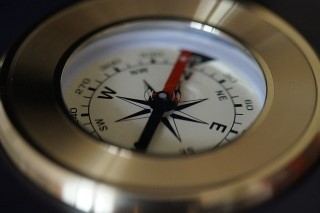
\includegraphics[width=0.5\columnwidth]{pictures/chapter11/compass.jpg}
\caption{나참판 (pixabay.com, 라이선스:CC0)}
\end{figure}

우리가 현재 편리하게 사용하고 있는 내비게이터는 비교적 역사가 짧은데 1981년 일본의 혼다에서 '일렉트로 자이로케이터(Electro Gryrocator)\footnote{\url{http://en.wikipedia.org/wiki/Electro_Gyrocator}}’ 라는 3축 자이ROS코프와 필름 지도를 기반으로 한 아날로그 방식이 처음 제안되었다(참고자료[2]). 그 후 미국 자동차용품업체 이택(Etak)의 전자 나침판과 바퀴에 센서를 장착하여 동작하는 전자식 내비게이션 ‘이택 내비게이터(Etak Navigator\footnote{\url{http://en.wikipedia.org/wiki/Etak}})’ 등이 나오기 시작했다. 그러나 전자 나침판과 바퀴에 센서를 장착하는 것은 비싼 자동차 가격에 더욱 부담이 되고 신뢰도에서도 문제가 있었다. 미국은 1970년대 부터 군사 목적으로 인공 위성을 이용한 위치 시스템을 개발하고 있었는데 2000년대에 그 중 24개의 GPS(Global Positioning System)\footnote{\url{http://en.wikipedia.org/wiki/Global_Positioning_System}} 위성을 개방하게 되었고 지금의 네비게이터 방식이 보급되기 시작하였다.

이야기를 로봇쪽으로 돌려보자. 로봇에도 이 네비게이션 기능이 사용된다면 얼마든지 우리 환경에서 활보하며 활약 할 수 있을 것이다. 이미, 로봇 공학에서는 가장 기본 중에 기본으로 네비게이션 분야는 꾸준히 연구되고 있고 발전을 거듭하고 있다. 로봇 공학에서 네비게이션은 빼놓을 수 없고 그 만큼 중요하다. 우리는 이 강좌를 시작으로 네비게이션에 대해 알아보기로 한다.

%-------------------------------------------------------------------------------
\subsection{땔래야 땔 수 없는 SLAM과 내비게이션(navigation)}

이 모바일 로봇의 기본이자 꽃은 바로 내비게이션이라고 할 수 있겠다. 내비게이션은 로봇이 정해진 목적지까지 이동하는 것으로, 말이야 쉽지만 로봇 자기 자신이 어디에 있는지, 그리고 주어진 환경의 지도를 가지고 있어야 한다는 것, 다양한 경로중에 최적화된 경로는 어떤 것인지, 그리고 도중에 로봇에게 장애물이 되는 벽, 가구, 물체 등을 피하여 이동하는 등 어디 하나 쉬운 미션이 하나도 없다. 

\begin{figure}[h]
\centering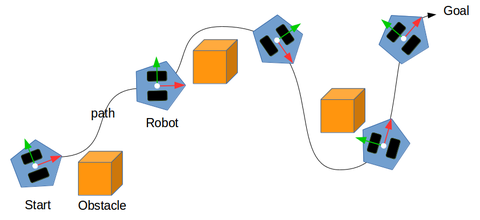
\includegraphics[width=0.8\columnwidth]{pictures/chapter11/navigation_concept.png}
\caption{내비게이션}
\end{figure}

로봇에 있어서 내비게이션을 위해서는 어떠한 것 들이 필요할까? 내비게이션 알고리즘에 따라 틀리겠지만 필수적으로는 아래의 기능 정도는 갖추고 있어야 할 것이다. 

① 지도
② 로봇의 위치 계측/추청하는 기능
③ 벽, 물체 등의 장애물의 계측하는 기능
④ 목적지까지의 최적 경로를 계산하고 주행하는 기능

예를 들어, 이해하기 쉽도록 로봇의 내비게이션 구성 요소와 자동차의 내비게이터를 비교해 보자.

첫 번째는 지도이다. 내비게이터는 구매시 부터 매우 정확한 지도가 탑재되어 있고 이 지도를 기반으로 목적지까지 안내 받을 수 있게 된다. 그러나, 서비스 로봇이 사용되는 실내에서 지도가 따로 있을까? 내비게이터와 마찬가지로 지도가 필요함으로 사람이 직접 지도를 작성하여 로봇에게 주던지, 로봇 스스로가 지도를 작성하여야 할 것이다. 로봇이 스스로 혹은, 약간의 인간의 도움을 받아 지도를 작성하기 위해서 등장한 것이 바로 SLAM(Simultaneous localization and mapping)\footnote{\url{http://en.wikipedia.org/wiki/Simultaneous_localization_and_mapping}}이다. 우리 말로는 "동시적 위치추정 및 지도 작성" 이라고 표현할 수 있겠다. 이는 로봇이 미지의 임의 공간을 이동하면서 주변을 센싱하며 현재 위치를 추정하는과 동시에 그 과정에서 지도를 작성하는 방법이다. 이 SLAM에는 다양한 방법이 있는데 좀 더 자세한 설명은 추후에 이어지는 강좌에서 설명하도록 하겠다.

\begin{figure}[h]
\centering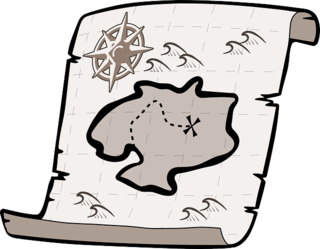
\includegraphics[width=0.3\columnwidth]{pictures/chapter11/treasure_map.png}
\caption{지도 (출처:pixabay.com, 라이선스:CC0)}
\end{figure}


두 번째로 로봇 스스로 위치를 계측/추정할 수 있어야 한다. 자동차의 경우 GPS 를 이용하여 자기 위치를 추정하지만, 실내에서는 GPS를 사용할 수 없고 만약에 사용할 수 있다고 하더라도 정밀한 이동을 위해서는 오차가 큰 GPS 는 쓸모가 없다. 그래서, 로봇은 일반적으로 자신이 움직이는 이동량을 바퀴의 회전축의 회전량을 가지고 측정하게 된다. 하지만, 바퀴의 회전량이라는게 추측 항법(dead reckoning\footnote{\url{http://en.wikipedia.org/wiki/Dead_reckoning}}\footnote{\url{http://www.cs.cmu.edu/afs/cs.cmu.edu/academic/class/16311/www/s07/labs/NXTLabs/Lab\%203.html}}, 데드레커닝)이라고 하여 오차가 꾀 발생한다. 그래서, IMU 센서 등으로 관성 정보를 취득하여 위치보상을 통해 그 오차를 줄여주는 방법이 사용되고는 한다.

\begin{figure}[h]
\centering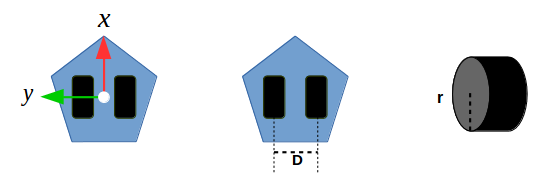
\includegraphics[width=0.9\columnwidth]{pictures/chapter11/deadreckoning.png}
\caption{데드레커닝에 필요한 정보(중심 위치, 바퀴나 거리, 바퀴 반지름)}
\end{figure}

추측 항법에 대해서 간략히 설명하겠다. 만약에, 위와 같이 로봇이 있을때, 바퀴간의 거리는 D, 바퀴의 반지름은 r 이락 하자. 그 후, 좌/우측 모터의 엔코더 값을 이용하여 수식(1)(2)(3)(4)로 변환 과정을 거치고 수식(5),(6)과 같이 로봇의 선속도(linear velocity: v)와 각속도(angular velocity: w)를 구할 수 있다. 그리고 최종적으로 Runge-Kutta 공식을 이용하여 식(7),(8), (9) 와 같이 이동한 위치, 각도의 근사값을 구할 수 있다.

\begin{figure}[h]
\centering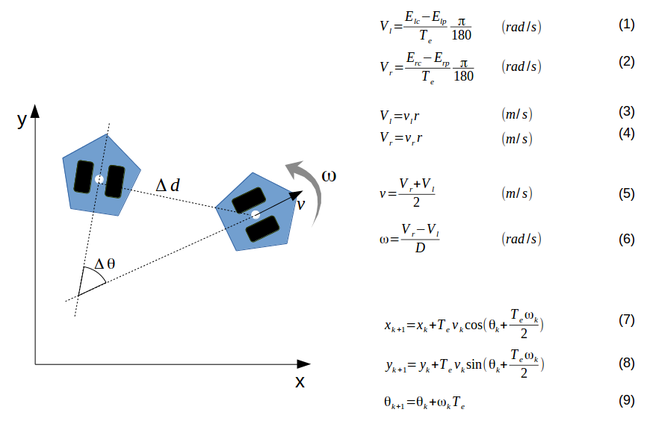
\includegraphics[width=\columnwidth]{pictures/chapter11/deadreckoning2.png}
\caption{추측 항법(deadreckoning)}
\end{figure}

세 번째로는 벽, 물체 등의 장애물을 파악하는 방법인데 이는 센서가 절대적으로 사용된다. 거리센서, 비전센서 등 다양한 종류의 센서가 사용되는데 거리센서는 LRF, 초음파센서, 적외선 거리센서 등이 사용되며 비전센서에는 스테레오 카메라, 모노카메라, 전방향 옴니 카메라, 그리고 최근에 Depth camera 로 많이 사용되는 Kinect, xtion 등이 장애물 파악하는데에 사용된다. 이 센서에 대한 내용은 대표적인 센서를 대상으로 이전 강좌로 설명하였다. 목차를 참고하여 보도록 하자.

네 번째로는 목적지까지의 최적 경로를 계산하고 주행하는 기능인데, 이것이 바로 이 강좌 처음에 말한 내비게이션(Navigation) 이다. 이는 경로 탐색/계획  (path search and planning)이라고 하는데 A* 알고리즘, 전자자기장 알고리즘, 파티클, 그래프 방식 등 매우 다양하다. 이 내용에 대해서는 추후 이어지는 강좌들에서 더 자세히 소개하도록 하겠다.

일단, 내비게이션 강좌가 시작된 샘이다. 내비게이션에 대해 간략히 정리를 해봤으나, 어렵고 방대한 내용이다. 네 가지 요소중에서 2번은 여기서 설명하였고, 3번은 이전 강좌에서 설명하였다. 이제 1번 SLAM과 2번 내비게이션대해서 추후 이어지는 강좌에서 부가적으로 자세히 설명하기로 하겠다.

%-------------------------------------------------------------------------------
\section{SLAM 실습편}\index{SLAM 실습편}
\label{sec:SlamExe}

%-------------------------------------------------------------------------------
\subsection{SLAM 따라하기}

SLAM에 대한 본 강좌에 앞서서 거북이를 이용하여 SLAM 하는 방법에 대해 설명하고 넘어가도록 하겠다. 아래의 따라하기식 강좌에서는 실제로 맵을 작성해 볼 수 있는 bag 파일도 첨부하니 한번 씩은 따라 해보는 것을 추천하고 싶다. SLAM 에 대한 이론 강좌는 추후 이어지는 강좌에서 이어서 설명하도록 하겠다.

%-------------------------------------------------------------------------------
\subsection{SLAM을 위한 로봇 하드웨어}

%-------------------------------------------------------------------------------
\subsubsection{제약사항}

본 강좌에서는 SLAM 중 오픈으로 공개 되어 있는 Gmapping\footnote{\url{https://www.openslam.org/gmapping.html}} (G. Grisetti, C. Stachniss, W, Burgard, CC BY-NC-SA 3.0))을 이용할 예정이다. 이는 몇 가지 하드웨어 제약을 가지고 있다. 일반적인 모바일 로봇의 경우에는 문제 없는 상황이지만 참고하길 바란다.

1) 이동 명령
두 축의 구동 모터로 이루어진 형태로 주로 좌/우축 바퀴가 따로 구동 가능한 차동 구동형 모바일 로봇(differential drive mobile robot) 또는, 옴니 휠 3개 이상의 구동축을 가지고 있는 전 방향 이동 로봇 (omni-wheel robot)과 같이 x, y, theta 속도 명령어로 받아 동작 가능해야 한다.

2) 주행기록계 (Odometry)
오도메트리 정보를 얻을 수 있어야 한다. 즉, 자신이 이동한 거리, 회전량을 추측 항법(dead reckoning, 데드레커닝)으로 계산 가능하거나, 이에 준하는 이동량을 구하기 위하여 IMU 센서 등의 관성 정보를 이용하여 위치 보상, 혹은, 단독으로 IMU 센서로 선속도(linear velocity)와 각속도(angular velocity)를 측정하여 로봇 스스로 자신의 위치를 계측/추청 가능해야 한다.

3) 계측 센서
SLAM과 내비게이션을 위하여 로봇은 X-Y 평면상의 장애물을 계측 가능한 LRF(Laser Range Finder), LiDAR 및 Kinect, Xtion 과 같은 Depth camera 의 경우에는 3차원 정보를 X-Y 평면상의 정보로 변환하여 사용 가능하다. 즉, 2차 평면 계측 가능 센서를 탑재하고 있어야 한다. 

(특별히 요구되지 않는 이상 초음파 센서 및 PSD 센서 등도 고려 대상이나 본 강좌에서는 다루지 않는다. 기타 카메라를 이용한 비쥬얼 SLAM 등은 본 강좌에서 다루지 않는다.)

4) 로봇 형태
직사각형 및 원형의 로봇만을 대상으로 한다. 한 쪽 축으로 길게 나온 변형의 로봇, 방문 사이로 지나가지 못할 정도로 너무 큰 로봇, 2족 휴머노이드 로봇, 다관절 로봇, 비행 로봇은 제외한다.

%-------------------------------------------------------------------------------
\subsubsection{사용되는 로봇과 센서}
\label{subsubsec:kobuki_robot_sensor}
본 강좌에서는 이전 강좌에 이어서 거북이 플랫폼\footnote{\url{http://wiki.ros.org/kobuki}}을 사용할 예정이다. 단, SLAM을 위하여 아래와 같이 기존 거북이 본체에 터틀봇2의 패키지로 제공하는 스택(검은색 판)과 폴(은색 스택 받침)을 2단으로 쌓았다. 1단에는 랩톱이 들어가 있으며, 그 위의 2단에는 Hokuyo LRF인 UTM-30LX, Depth camera 인 Kinect 과 Xtion 이 각각 올라간다. 이는 조금 전에 언급한 SLAM 제약 사항을 모두 만족하는 조건이다. 본 강좌에서는 LRF 센서를 이용한 아래의 좌측 그림과 같은 로봇을 이용하여 설명할 예정이다. 내비게이션 강좌가 모두 끝나면 Kinect, Xtion 등도 추가로 설명하도록 하겠다.

\begin{figure}[h]
\centering
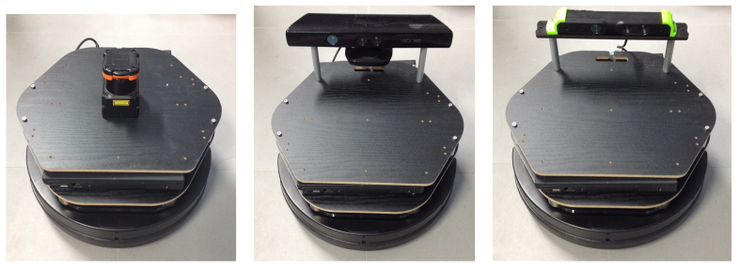
\includegraphics[width=0.9\columnwidth]{pictures/chapter11/kobuki_sensors.png}
\caption{LRF, Kinect, Xtion}
\end{figure}

%-------------------------------------------------------------------------------
\subsection{SLAM 계측 대상 환경}
\label{subsubsec:kobuki_target_environment}

SLAM 이 가능한 환경은 딱히 특정짓지는 않지만, Gmapping 의 알고리즘 상 특징 요소가 매우 적은 1) 장애물 하나도 없는 정사각 형태의 환경, 2) 장애물 하나 없이 양 벽이 평행하게 길게 이어진 복도, 3) 레이저 및 적외선이 반사되지 못하는 유리창 및 4) 산란되는 거울, 5) 호수, 바닷가 등의 경우 및 사용하는 센서의 특성에 따라 장애물 정보를 취득 못하는 환경은 제외된다.

이번 강좌에서는 필자의 연구실에 마련된 실험 공간을 타겟 환경으로 정했다. 이 환경은 일반 가정집을 가정하여 침대, 책상, 테이블, 선반, 책장, 냉장고, TV, 소파 등으로 구성되어 있다. 아래에 실험 환경의 실제 사진과 3차원 정보를 첨부 사진으로 올렸으니 참고하기 바란다. 

\begin{figure}[h]
\centering
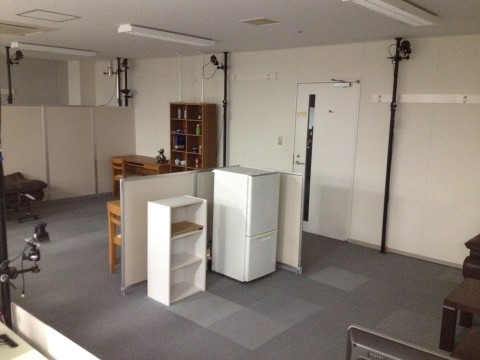
\includegraphics[height=40mm]{pictures/chapter11/room.jpg}
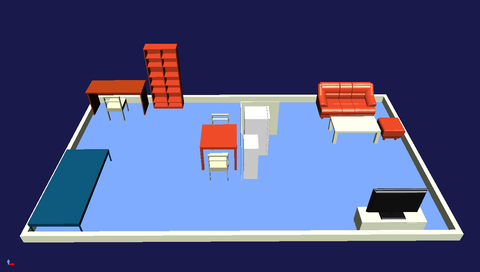
\includegraphics[height=40mm]{pictures/chapter11/room_choreonoid.png}
\caption{좌측: 계측 대상 환경, 우측: 오픈소스 로봇 시뮬레이터인 choreonoid 에서 본 계측 대상 환경}
\end{figure}

%-------------------------------------------------------------------------------
\subsection{SLAM을 위한 ROS 패키지}

본 강좌에서 사용할 SLAM 관련 ROS 패키지는 kobuki 메타 패키지와 slam\_gmappig 메타 패키지의 gmapping 패키지, navigation 메타 패키지의 map\_server 패키지 이다. 아래와 같이 미리 모두 설치해 두도록 하자. 본 강좌는 따라하기 강좌이기에 때문에 실행 방법만을 기술할 예정이다. 각 패키지의 설명은 다음 강좌에서 매우 자세히 다루도록 하겠다. 

\noindent
※ 이번 강좌 부터는 작업 혼란을 막기 위하여, 모든 패키지를 거북이에 설치하고 진행하도록 하겠다. 패키지의 설치, 각 노드, 런치파일의 실행은 모두 거북이 본체와 연결된 랩톱에서 실행해야 한다.

\vspace{\baselineskip}
\begin{lstlisting}[language=ROS]
$ sudo apt-get install ros-indigo-kobuki*
$ sudo apt-get install ros-indigo-gmapping
$ sudo apt-get install ros-indigo-navigation
\end{lstlisting}

\noindent
센서 패키지로는 사용하는 센서에 맞도록 관련 패키지를 아래와 같이 설치하도록 하자.

\setcounter{num}{0}

\vspace{\baselineskip}
\noindent
\stepcounter{num}
\thenum) Hokuyo LRF\footnote{\url{https://www.hokuyo-aut.jp/02sensor/07scanner/utm_30lx.html}} (URG-04LX 및 UTM-30LX 시리즈)
\begin{lstlisting}[language=ROS]
$ sudo apt-get install ros-indigo-urg-node
\end{lstlisting}
 
\vspace{\baselineskip}
\noindent
\stepcounter{num}
\thenum) Kinect
\begin{lstlisting}[language=ROS]
$ sudo apt-get install ros-indigo-openni-camera ros-indigo-openni-launch
\end{lstlisting}


\vspace{\baselineskip}
\noindent
\stepcounter{num}
\thenum) Xtion
\begin{lstlisting}[language=ROS]
$ sudo apt-get install ros-indigo-openni2-camera ros-indigo-openni2-launch
\end{lstlisting}


%-------------------------------------------------------------------------------
\subsection{SLAM 실행}

※ 현재 아래의 강좌는 거북이와 LRF 를 이용한 강좌이다. Kinect 및 Xtion 의 경우에는 추후에 추가하도록 하겠다.

\setcounter{num}{0}

\vspace{\baselineskip}
\noindent
\stepcounter{num}
\thenum) 소스 다운로드 및 컴파일\\
우선, 오로카 Github 주소에서 관련 패키지를 다운로드 받는다. 그 후, 컴파일을 해준다.
\vspace{\baselineskip}
\begin{lstlisting}[language=ROS]
$ cd ~/catkin_ws/src
$ git clone https://github.com/oroca/oroca-ros-pkg.git
$ cd ~/catkin_ws && catkin_make
\end{lstlisting}

\vspace{\baselineskip}
\noindent
\stepcounter{num}
\thenum) 거북이 노드 실행\\
roscore 를 실행한 후, 거북이 노드를 실행한다.

\vspace{\baselineskip}
\begin{lstlisting}[language=ROS]
$ roscore

$ roslaunch kobuki_node minimal.launch --screen
\end{lstlisting}

\vspace{\baselineskip}
\noindent
\stepcounter{num}
\thenum) kobuki\_slam 실행\\
kobuki\_slam 패키지는 단순히 런치 파일 하나로만 구성되어 있다. 이 런치 파일은 LRF의 드라이버인 urg\_node 노드, 좌표 변환을 위한 tf 를 활용한 kobuki\_tf 노드, 맵 작성을 위해 slam\_gmapping 노드를 포함하여 총 3개의 노드가 함께 실행된다.
\vspace{\baselineskip}
\begin{lstlisting}[language=ROS]
$ sudo chmod a+rw /dev/ttyACM0
$ roslaunch kobuki_slam kobuki_slam.launch
\end{lstlisting}

\vspace{\baselineskip}
\noindent
\stepcounter{num}
\thenum) RViz 실행\\
SLAM 도중 결과를 눈으로 확인 할 수 있도록 ROS 의 시각화툴인 RViz를 구동하도록 하자. 구동 시에 아래와 같이 옵션을 붙여주면 디스플레이 플러그인들이 처음부터 추가되어 매우 편리하다.
\vspace{\baselineskip}
\begin{lstlisting}[language=ROS]
$ rosrun rviz rviz -d `rospack find kobuki_slam`/rviz/kobuki_slam.rviz
\end{lstlisting}

\noindent
\stepcounter{num}
\thenum) 토픽 데이터 저장\\
6번에서 유저가 직접 로봇을 조정하며 SLAM 작업을 하게 되는데 이때에 kobuki 와 kobuki\_slam 패키지에서 발행하는 /scan과 /tf 토픽을 scan\_data 이라는 파일명의 bag 파일로 저장하게 된다. 나중에 이 파일을 가지고 맵을 만들 수도 있고 실험할때의 작업을 반복하지 않아도 맵핑작업시에 실험 당시의 /scan과 /tf 토픽 을 재현할 수 있다. 실험을 녹음한다고 생각하면 된다.

\vspace{\baselineskip}
\begin{lstlisting}[language=ROS]
$ rosbag record -O scan_data /scan /tf
\end{lstlisting}

\vspace{\baselineskip}
\noindent
\stepcounter{num}
\thenum) 로봇 조종\\
아래의 명령어로 유저가 직접 로봇을 조정하며 SLAM 작업을 한다. 여기서 중요한 점은 로봇의 속도를 너무 급하게 바꾸거나 너무 빠른 속도로 전/후진, 회전하지 않도록 주의한다. 그리고, 로봇을 이동시킬 때 계측할 환경의 구석 구석을 로봇이 돌아다니며 스캔할 필요가 있다. 이 부분은 경험이 필요한 부분이니 위 SLAM 작업을 많이 해보며 경험을 쌓아보도록 하자. 

\vspace{\baselineskip}
\begin{lstlisting}[language=ROS]
$ roslaunch kobuki_keyop safe_keyop.launch
\end{lstlisting}

\vspace{\baselineskip}
\noindent
\stepcounter{num}
\thenum) 로봇 조종\\
로봇을 이동시키면 로봇의 오도메트리, tf 정보, 센서의 스캔 정보를 기반으로 맵이 작성된다. 이는 위에서 실행한 RViz 에서 확인 가능하다. 모든 작업이 완료 되었으며 map\_saver 노드를 실행하여 맵을 작성하자. 작성된 맵은 map\_saver를 동작시킨 디렉토리에 저장되며 파일명은 특명히 지정해주지 않는 이상 실제 맵인 map.pgm 파일명과 맵 정보가 포함된 map.yaml 파일명으로 저장된다.
\vspace{\baselineskip}
\begin{lstlisting}[language=ROS]
$ rosrun map_server map_saver
\end{lstlisting}

\noindent
1번에서 7번의 과정을 통하여 맵을 작성할 수 있다. 그 과정을 아래의 그림으로 나타내며, 그 결과물인 지도를 아래에 함께 첨부한다. 위 에서 언급한 실험 환경의 맵이 제대로 작성되었음을 확인 할 수 있다.

\begin{figure}[h]
\centering
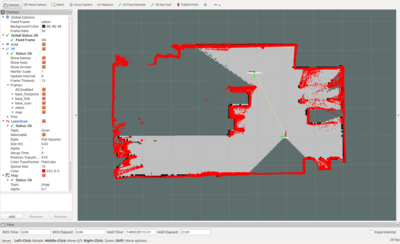
\includegraphics[width=0.5\columnwidth]{pictures/chapter11/slamtest1.png}
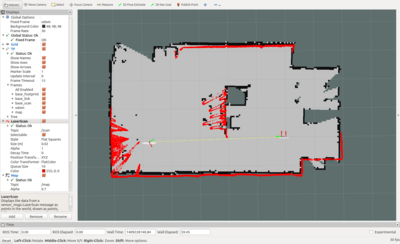
\includegraphics[width=0.5\columnwidth]{pictures/chapter11/slamtest2.png}
\caption{지도 작성을 위한 SLAM이 실행되고 있는 모습}
\end{figure}

\begin{figure}[h]
\centering
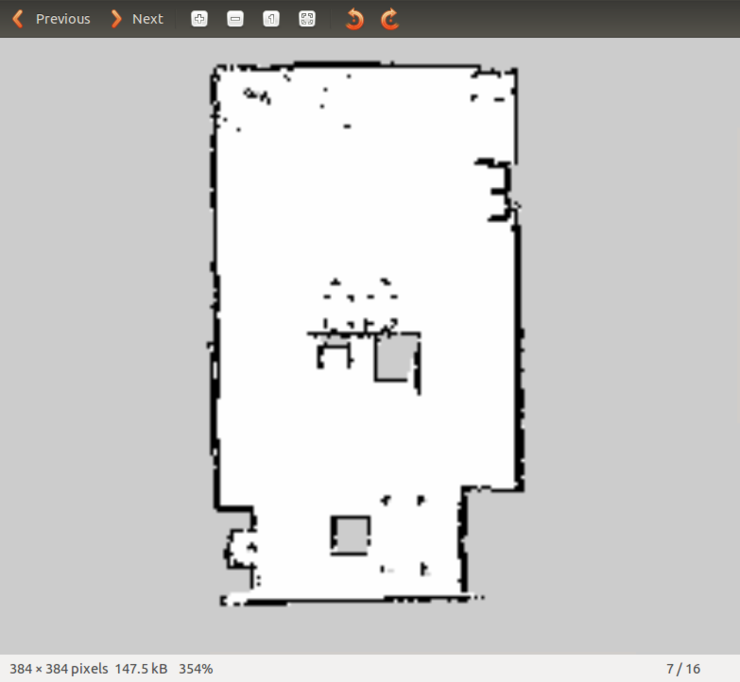
\includegraphics[width=0.7\columnwidth]{pictures/chapter11/slamtest_map.png}
\caption{완성된 지도}
\end{figure}

%-------------------------------------------------------------------------------
\subsection{미리 준비된 bag 파일을 이용한 SLAM}

아래의 내용은 거북이 및 LRF 센서 없이도 SLAM 을 접해 볼 수 있도록 위에서 녹화해둔 bag 파일로 직접 해보기로 하겠다. 우선, 본 강좌의 첨부파일을 다운로드 하자. 압축되어 있으니 이를 해제한 후 자신의 ~/ 폴더에 넣도록 하자. 그 다음에 내용은 위에서 SLAM 실행 방법과 일치한다. 다만, rosbag 만 저장이 아닌 재생(play) 를 하여 실제 실험하는 것과 동일하게 동작 할 것이다. 다만, 여기서 주의 할점은 파라매터 중 use\_sim\_time 를 활성화 시켜서 현재 시간이 아닌 bag 파일이 저장되었던 시점의 시간을 이용해야 문제가 없다. 직접 해보기를 추천한다.

\vspace{\baselineskip}
\begin{lstlisting}[language=ROS]
$ roscore
$ rosparam set use_sim_time true
$ roslaunch kobuki_slam kobuki_slam_demo.launch
$ rosrun rviz rviz -d `rospack find kobuki_slam`/rviz/kobuki_slam.rviz
$ rosbag play ./scan_data.bag
$ rosrun map_server map_saver
\end{lstlisting}

다음 강좌에서는 위에서 실행했던 패키지들의 자세한 소스 설명 및 설정법에 대해서 추가 설명을 하도록 하자.

\newpage
%-------------------------------------------------------------------------------
\section{SLAM 응용편}\index{SLAM 응용편}
\label{sec:SlamApp}

섹션~\ref{sec:SlamExe}~\nameref{sec:SlamExe}(pp.\pageref{sec:SlamExe})이 단순히 따라해보는 강좌였다면 이번 강좌에서는 SLAM 에서 사용되는 ROS 패키지를 자세히 살펴보고 어떻게 작성, 설정하는지에 대해서 알아 보는 응용편이라고 할 수 있다. 즉, kobuki 메타 패키지와 slam\_gmappig 메타 패키지의 gmapping 패키지, navigation 메타 패키지의 map\_server 패키지 를 자세히 살펴볼 예정이다. 이는 앞서 진행한 서브섹션~\ref{sec:SlamExe}~\nameref{sec:SlamExe}(pp.\pageref{sec:SlamExe})을 자신의 로봇에 적용해 볼 수 있는 응용편이라고 볼 수 있다. SLAM 자체에 대한 이론적인 설명은 섹션~\ref{sec:SlamTheory}~\nameref{sec:SlamTheory}(pp.\pageref{sec:SlamTheory}) SLAM 이론편에서 설명하도록 하겠다.
\label{sec:SlamTheory}
이 과정에서 본 강좌는 거북이라는 플랫폼과 LRF 센서를 기반으로 설명하겠지만, 이를 응용하면 특정 로봇 플랫폼, 특정 센서에 국한되지 않고 자신만의 로봇으로 SLAM 이 가능하게 될 것이다. 자신만의 로봇 플랫폼을 만들거나 거북이 로봇 플랫폼 위에 자신만의 스타일로 새로운 로봇을 구성하고 싶다면 이 강좌가 도움이 될 것이다.

%-------------------------------------------------------------------------------
\subsection{지도 (map)}

우선, 우리가 이 강좌에서 궁긍적으로 얻고자 하는 출력 물이 지도라는 점에서 지도에 대해 알고 넘어가야할 듯 싶다. 우리 인간이 사용하고 있는 종이 지도를 준다고 해도 로봇이 이를 이해할까? 그렇지는 않을 것이다. 로봇이 이해하기 편하고 계산하기 쉽게 만들어서 디지털 파일로 줘야 할 것이다. 이러한 로봇 내비게이션 지도에 대한 정의는 오래전 부터 많이 논의되고 있고 지금도 끝이지 않고 있다. 특히, 최근에는 2차원뿐 아니라 3차원 정보까지 포함하거나, 단지 이동과 관련된 정보뿐만 아니라 각 물체에 대한 세그멘테이션 등이 포함된 지도도 있다.

이번 강좌에서는 ROS 커뮤니티에서 일반적으로 많이 사용되는 2차원 점유 격자 지도(OGM, Occupancy Grid Map\footnote{\url{http://en.wikipedia.org/wiki/Occupancy_grid_mapping}})를 이용할 것이다. 이 전 강좌에서 얻을 수 있었던 아래의 그림과 같은 지도를 말하는 것으로 흰색은 로봇이 이동 가능한 자유 영역 (free area), 검은색은 이동 불가능한 점유 영역 (occupied area), 회색은 확인되지 않은 미지 영역 (unknown area) 으로 표현된다. 이 영역들은 0에서 255의 값으로 표현하는 그레이스케일(gray scale) 값으로 나타낸다. 이 값은 점유 상태(occupancy state)를 표현한 점유 확률(occupancy probability)을 베이즈(Bayes)정리의 사후 확률(posterior probability)을 통해 구하게 된다. 점유 확률 occ 는 occ = (255 - color\_avg) / 255.0 으로 표현된다. 만약, 이미지가 24비트라면 color\_avg = ( 한 셀의 그레이스케일 값 / 0xFFFFFF * 255 ) 이 된다. 이 occ 가 1에 가까울 수록 점유되었을 확률이 높아지고 0 에 가까울 수록 비 점유되었다는 것을 의미한다.

ROS 의 메시지(nav\_msgs/OccupancyGrid)로 발행될 때는 이를 다시 재정의하여 점유도를 정수 [0 ~ 100] 까지로 표현하고 있다. "0"에 가까울 수록 이동 가능한 자유 영역 (free area), "100"에 가까울 수록 이동 불가능한 점유 영역 (occupied area), 그리고 "-1" 은 특별히 확인되지 않은 미지 영역 (unknown area)으로 정의하고 있다.

\begin{figure}[h]
\centering
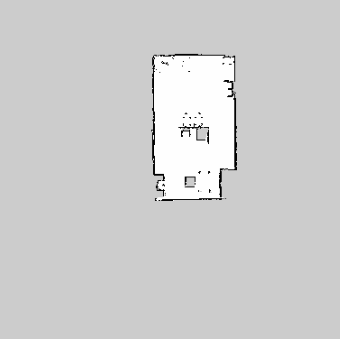
\includegraphics[width=0.7\columnwidth]{pictures/chapter11/slam_map.png}
\caption{완성된 점유 격자 지도}
\end{figure}


ROS 에서는 지도 정보를 portable graymap format 이라고 하는 *.pgm\footnote{\url{http://en.wikipedia.org/wiki/Netpbm_format}} 파일 형태를 저장/이용하고 있다. 또한, *.yaml 을 함께 포함하고 있어서 여기에 맵의 정보를 기재한다. 예를들어, 우리가 이전 강좌에서 작성한 지도의 정보를 확인하면 아래와 같은데 image 은 파일명, resolution은 지도의 해상도로 meters / pixel 단위이다.

즉 아래의 경우, 각 픽셀은 5cm 를 의미한다. origin은 지도의 원점으로 각 숫자는 각각 x, y, yaw 를 의미한다. 즉, 위 지도의 왼쪽 하단이 x = -10미터, y = -10미터 이다. negate 은 흑/백을 반전하게 된다. 그리고, 각 필셀의 흰색/흑색의 결정은 점유 확률(occupancy probability)이 occupied\_thresh 한계치를 넘으면 검은색인 이동 불가능한 점유 공간 (occupied area)으로 표현하며, free\_thresh 보다 작으면 반대로 흰색인 이동 가능한 자유 공간 (free area) 으로 표현한다.

\vspace{\baselineskip}
\vspace{\baselineskip}
\begin{lstlisting}[language=ROS]
image: map.pgm
resolution: 0.050000
origin: [-10.000000, -10.000000, 0.000000]
negate: 0
occupied_thresh: 0.65
free_thresh: 0.196
\end{lstlisting}


%-------------------------------------------------------------------------------
\subsection{SLAM 에 필요한 정보}

지도에 대해 알아봤으니 이 지도 작성을 위한 재료들에 대해서 알아 보기로 하자! 우선, 각자 생각해 보기로 하는데 아래의 물음에 대답할 수 있는가?. 


"지도를 작성할 때 뭐가 필요할까?" 



답부터 말하면 제일 먼저 필요한 것은 1) 거리 값이다. "나를 중심으로 저기에 있는 소파는 2미터 떨어져 있다"라고 판단할 수 있는 거리 값을 의미한다. 이는 LRF, Depth camera 등의 센서를 이용하여 X-Y평면상을 스캔한 값이라고 볼 수 있다.

두 번째는 나의 2) 위치 값이다. "나"라고 하면 여기서는 "센서"를 말하고, 이 센서의 위치는 로봇에 고정되어 있기 때문에 로봇이 움직이면 센서도 함께 움직인다. 그러니 센서의 위치 값은 로봇의 이동량인 오도메트리(odometry)에 의존하게 된다. 이를 계산하여 위치 값으로 제공할 필요가 있다.

여기서 언급한 거리 값은 ROS 에서는 scan 이라는 이름으로 부르며, 위치 정보는 의존 관계에 따라 바뀌기 때문에 tf 라는 이름으로 부른다. (참고로 tf는 변환이라는 의미로 위치 정보 변환,  연결축 변환 등에 사용된다.) 이 scan과 tf 의 2 가지 정보를 기반으로 SLAM 실행하게 되고 우리가 원하는 지도를 작성할 수 있게 된다. 

\begin{figure}[h]
\centering
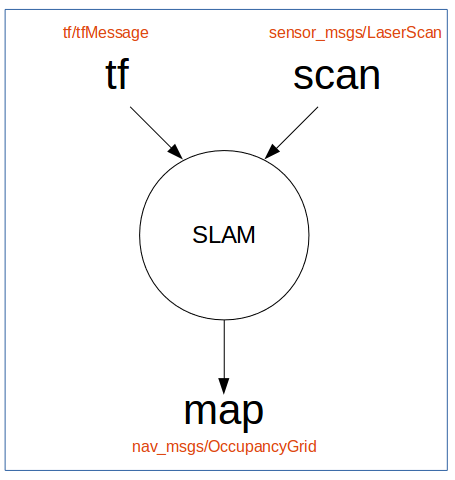
\includegraphics[width=0.6\columnwidth]{pictures/chapter11/tf_scan_slam_map.png}
\caption{SLAM에 필요한 tf와 scan 데이터와 그 결과로서의 map의 관계}
\end{figure}

%-------------------------------------------------------------------------------
\subsection{kobuki\_slam의 기능과 처리 과정}

필자는 지도를 작성하기 위하여 kobuki 노드 이외에 추가적으로 SLAM을 위하여 kobuki\_slam 패키지를 만들었다. 이 패키지는 소스 파일은 없지만 slam 에 필요한 패키지를 launch 파일로 묶어서 실행하고 있다. 이 과정을 그림을 설명하면 아래의 그림과 같다.  

\setcounter{num}{0}

\vspace{\baselineskip}
\noindent
\stepcounter{num}
\thenum) kobuki\_urg\_node\\
LRF 센서를 실행하여 SLAM 에 필요한 scan 정보를 slam\_gmapping 노드에게 보낸다. 이는 단 한번으로 끝나지 않고 로봇이 움직이더라도 지속적으로 scan 정보를 보내게 된다.

\vspace{\baselineskip}
\noindent
\stepcounter{num}
\thenum) kobuki\_keyop\\
키보드 입력 값을 받아서 로봇을 조종 가능한 노드이다. 거북이 노드에게 이동 속도, 회전 속도 명령을 보낸다.

\vspace{\baselineskip}
\noindent
\stepcounter{num}
\thenum) kobuki\_node\\
거북이 노드는 유저의 명령을 받고 이동하게 된다. 이 때에 내부적으로는 자신의 위치를 계측/측정한 위치 정보인 odom 정보를 전송하는가 동시에 같은 이름으로 odom 의 위치 변환 정보를 tf 로 내보내며, 이와 연결된 로봇의 중앙 부분의 base\_footprint 위치도 tf로 내보내게 된다.

\vspace{\baselineskip}
\noindent
\stepcounter{num}
\thenum) kobuki\_tf\\
kobiki\_tf 에서는 센서의 위치인 base\_scan 을 tf 형태로 SLAM에게 넘기기 위하여 odom → base\_footprint → base\_link → base\_scan 의 변환을 거쳐서 내보낸다.

\vspace{\baselineskip}
\noindent
\stepcounter{num}
\thenum) slam\_gmapping\\
slam\_gmapping 노드에서는 센서가 측정한 1) 거리 값 인 scan 정보와 센서의 2) 위치 값 인 tf 정보를 기반으로 지도를 작성하게 된다. 

\vspace{\baselineskip}
\noindent
\stepcounter{num}
\thenum) map\_saver\\
map\_server 패키지의 map\_saver 노드는 이 지도 정보를 가지고 저장 가능한 map.pgm 파일과 이에 대한 정보 파일인 map.yaml 파일을 생성하게 된다.

\begin{figure}[h]
\centering
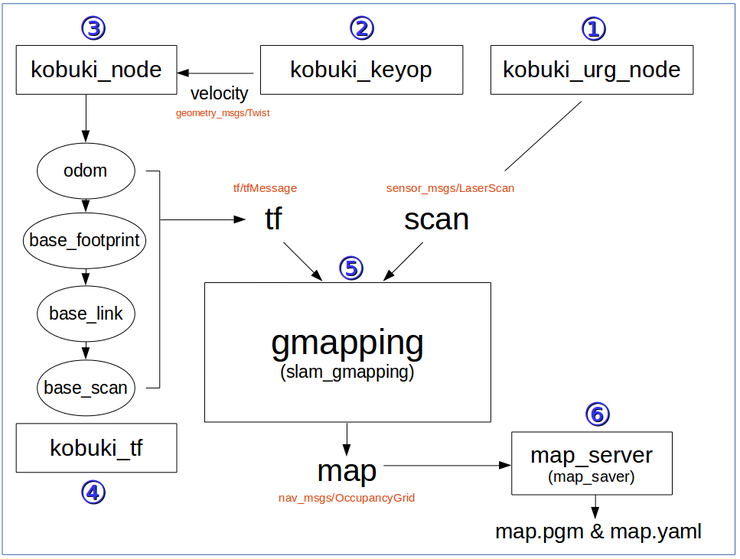
\includegraphics[width=\columnwidth]{pictures/chapter11/slam_flow.png}
\caption{kobuki\_slam 흐름도}
\end{figure}

%-------------------------------------------------------------------------------
\subsection{로봇 각 부분의 상대 위치 변환 정보 (tf)}

상대 위치 변환 정보를 시각화를 통하여 알아보면 아래의 그림과 같이 나타낼 수 있다. 그림이 상당히 크게 나왔는데 클릭하여 큰 원본 파일을 볼 수 있도록 하였다. 이 정보를 알고 있어야 뒤에 있는 kobuki\_tf 및 kobuki\_slam 패키지를 만들 수 있다. 위 그림은 "rosrun rqt\_tf\_tree rqt\_tf\_tree" 통해 확인 할 수 있는 tf\footnote{\url{http://wiki.ros.org/tf}} 의 tree 뷰어이고, 아래의 그림은 "rosrun rviz rviz" 에서 "tf" 플러그인을 추가하면 확인한 tf 정보이다. 

즉, odom → base\_footprint → base\_link → base\_scan 순으로 위치 정보가 연관되어 있다. 우리가 SLAM 에서는 이 모든 tf 정보가 필요하다.

\begin{figure}[h]
\centering
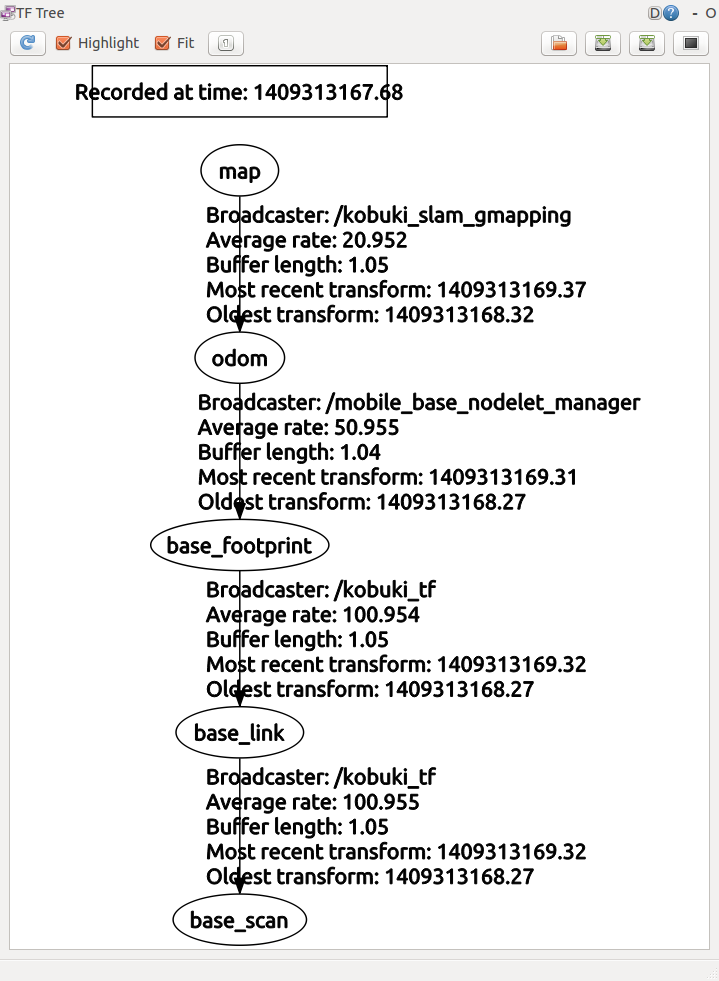
\includegraphics[width=0.6\columnwidth]{pictures/chapter11/slam_tf.png}
\caption{로봇 각 부분의 상대 위치 변환 정보}
\end{figure}

\newpage
%-------------------------------------------------------------------------------
\subsection{kobuki\_tf 패키지 작성}

\setcounter{num}{0}

\vspace{\baselineskip}
\noindent
\stepcounter{num}
\thenum) 패키지 생성
\begin{lstlisting}[language=ROS]
$ cd ~/catkin_ws/src/
$ catkin_create_pkg kobuki_tf roscpp tf geometry_msgs
\end{lstlisting}


\vspace{\baselineskip}
\noindent
\stepcounter{num}
\thenum) 소스파일 생성 및 수정
\begin{lstlisting}[language=ROS]
$ gedit kobuki_tf/src/tf_broadcaster.cpp 
\end{lstlisting}

\vspace{\baselineskip}
\begin{lstlisting}[language=C++]
#include <ros/ros.h>
#include <tf/transform_broadcaster.h>

int main(int argc, char** argv){
  ros::init(argc, argv, "kobuki_tf");
  ros::NodeHandle n;

  ros::Rate r(100);

  tf::TransformBroadcaster broadcaster;

  while(n.ok()){
    broadcaster.sendTransform(
      tf::StampedTransform(
        tf::Transform(
          tf::Quaternion(0, 0, 0, 1),
          tf::Vector3(0.0, 0.0, 0.01)),
          ros::Time::now(),
          "base_footprint",
          "base_link"));

    broadcaster.sendTransform(
      tf::StampedTransform(
        tf::Transform(
          tf::Quaternion(0, 0, 0, 1),
          tf::Vector3(0.0, 0.0, 0.24)),
          ros::Time::now(),
          "base_link",
          "base_scan"));

    r.sleep();
  }
}
\end{lstlisting}

\noindent
kobuki\_node 에서는 odom → base\_footprint 의 tf 를 제공한다. 이 kobuki\_tf 에서는 여기에 이어서 base\_link 와 base\_scan 를 추가해 주겠다.\\


odom → base\_footprint  → base\_link → base\_scan

\vspace{\baselineskip}
\noindent
위와 같이 만들어 주기 위해서는 센서 위치인 base\_scan 를 알아야 한다. 이 위치 정보 변환을 위하여 base\_link 는 바닥(base\_footprint)으로부터 0.01m (1cm) 위에 있고, 센서 위치인 base\_scan 은 base\_link 로부터 0.24m (24cm)에 위치해 있다는 것을 위의 소스에 반영하였다.

\vspace{\baselineskip}
\noindent
\stepcounter{num}
\thenum) CMakeLists.txt 설정

\vspace{\baselineskip}
\begin{lstlisting}[language=ROS]
$ gedit kobuki_tf/CMakeLists.txt 
\end{lstlisting}

\begin{lstlisting}[language=make]
add_executable(kobuki_tf src/tf_broadcaster.cpp)
target_link_libraries(kobuki_tf ${catkin_LIBRARIES})
\end{lstlisting}

\noindent
위 두 가지 설정을 추가하는 것으로 "kobuki\_tf" 라는 실행 파일을 생성할 수 있게 된다.

\vspace{\baselineskip}
\noindent
\stepcounter{num}
\thenum) 컴파일

\vspace{\baselineskip}
\begin{lstlisting}[language=ROS]
$ cd ~/catkin_ws && catkin_make
\end{lstlisting}



%-------------------------------------------------------------------------------
\subsection{kobuki\_slam 패키지 작성}

\setcounter{num}{0}

\vspace{\baselineskip}
\noindent
\stepcounter{num}
\thenum) 패키지 생성 및 launch 파일 폴더 생성

\vspace{\baselineskip}
\begin{lstlisting}[language=ROS]
$ cd ~/catkin_ws/src/
$ catkin_create_pkg kobuki_slam roscpp kobuki_node urg_node
$ mkdir kobuki_slam/launch
\end{lstlisting}


\vspace{\baselineskip}
\noindent
\stepcounter{num}
\thenum) 소스파일 생성 및 수정

\begin{lstlisting}[language=ROS]
$ gedit kobuki_slam/launch/kobuki_slam.launch
\end{lstlisting}

\vspace{\baselineskip}
\begin{lstlisting}[language=XML]
<launch>
  <node pkg="urg_node" type="urg_node" name="kobuki_urg_node" output="screen">
    <param name="frame_id" value="base_scan" />
  </node>

  <node pkg="kobuki_tf" type="kobuki_tf" name="kobuki_tf" output="screen"></node>

  <node pkg="gmapping" type="slam_gmapping" name="kobuki_slam_gmapping" output="screen">
    <param name="base_frame" value="base_footprint"/>
    <param name="odom_frame" value="odom"/>
    <param name="map_update_interval" value="1.0"/>
    <param name="maxUrange" value="6.0"/>
    <param name="sigma" value="0.05"/>
    <param name="kernelSize" value="1"/>
    <param name="lstep" value="0.05"/>
    <param name="astep" value="0.05"/>
    <param name="iterations" value="5"/>
    <param name="lsigma" value="0.075"/>
    <param name="ogain" value="3.0"/>
    <param name="lskip" value="0"/>
    <param name="srr" value="0.01"/>
    <param name="srt" value="0.02"/>
    <param name="str" value="0.01"/>
    <param name="stt" value="0.02"/>
    <param name="linearUpdate" value="0.25"/>
    <param name="angularUpdate" value="0.25"/>
    <param name="temporalUpdate" value="-1.0"/>
    <param name="resampleThreshold" value="0.5"/>
    <param name="particles" value="300"/>
    <param name="xmin" value="-10.0"/>
    <param name="ymin" value="-10.0"/>
    <param name="xmax" value="10.0"/>
    <param name="ymax" value="10.0"/>
    <param name="delta" value="0.05"/>
    <param name="llsamplerange" value="0.01"/>
    <param name="llsamplestep" value="0.01"/>
    <param name="lasamplerange" value="0.005"/>
    <param name="lasamplestep" value="0.005"/>
    </node>
</launch>
\end{lstlisting}



\vspace{\baselineskip}
\noindent
\thenum-1) kobuki\_urg\_node 노드 설정
아래의 내용은 거북이에 장착되어 있는 LRF 를 구동하기 위한 구문으로 "frame\_id" 파라미터를 "base\_scan" 으로 변환시켜 실행시키도록 한다.

\vspace{\baselineskip}
\begin{lstlisting}[language=XML]
  <node pkg="urg_node" type="urg_node" name="kobuki_urg_node" output="screen">
    <param name="frame_id" value="base_scan" />
  </node>
\end{lstlisting}

\vspace{\baselineskip}
\noindent
\thenum-2) kobuki\_tf 노드 설정
이 런치 파일을 수행하게 되면 좀전에 작성한 kobuki\_tf 를 함께 실행하게 된다.

\vspace{\baselineskip}
\begin{lstlisting}[language=XML]
  <node pkg="kobuki_tf" type="kobuki_tf" name="kobuki_tf" output="screen">
  </node>
\end{lstlisting}

\vspace{\baselineskip}
\noindent
\thenum-3) slam\_gmapping 노드 설정
slam\_gmapping 를 실행하게 되는데 다양한 옵션을 자신의 로봇과 센서에 맞도록 수정할 필요가 있다. 각 옵션은 아래와 같으니 참고하기 바란다.

\vspace{\baselineskip}
\begin{lstlisting}[language=XML]
<param name="base_frame" value="base_footprint"/> %*로봇 기본 프레임*)
<param name="odom_frame" value="odom"/>  %*오도메트리 프레임*)
<param name="map_update_interval" value="1.0"/> %*지도 갱신 시간 간격 (sec)*)
<param name="maxUrange" value="6.0"/>  %*최대 사용 가능한 레이저 거리 (meter)*)
<param name="sigma" value="0.05"/>  %*SLAM 에 사용되는 종단점 매칭 시그마 상수 값*)
<param name="kernelSize" value="1"/>  %*유관성 관련 커널 사이즈*)
<param name="lstep" value="0.05"/>  %*이동(translation) 최적화*)
<param name="astep" value="0.05"/> %*회전(rotation) 최적화*)
<param name="iterations" value="5"/> %*스캔매칭 반복 수*)
<param name="lsigma" value="0.075"/> %*우도(likelihood)계산에 필요한 시그마 값*)
<param name="ogain" value="3.0"/>  %*리샘플링 스므즈님을 위한 우도 평가의 게인 값*)
<param name="lskip" value="0"/>  %*각 스캔에서 넘어가는 빔의 수*)
<param name="srr" value="0.01"/>  %*오도메트리 에러 (이동 → 이동)*)
<param name="srt" value="0.02"/> %*오도메트리 에러 (이동 → 회전)*)
<param name="str" value="0.01"/>  %*오도메트리 에러 (회전 → 이동)*)
<param name="stt" value="0.02"/>  %*오도메트리 에러 (회전 → 회전)*)
<param name="linearUpdate" value="0.25"/> %*각 스캔 시간에서의 이동 업데이트*)
<param name="angularUpdate" value="0.25"/>  %*각 스캔 시간에서의 회전 업데이트*)
<param name="temporalUpdate" value="-1.0"/>  %*스캔보다 업데이트가 늦을때의 업데이트*)
<param name="resampleThreshold" value="0.5"/>  %*리샘플 한계치 값*)
<param name="particles" value="300"/>  %*파티클의 수*)
<param name="xmin" value="-10.0"/>  %*초기 최소 지도 크기 x*)
<param name="ymin" value="-10.0"/> %*초기 최소 지도 크기 y*)
<param name="xmax" value="10.0"/> %*초기 최대 지도 크기 x*)
<param name="ymax" value="10.0"/> %*초기 최대 지도 크기 y*)
<param name="delta" value="0.05"/>  %*지도의 해상도: 지도의 각 필셀당 거리*)
<param name="llsamplerange" value="0.01"/> %*우도를 위한 이동 샘플링 거리*)
<param name="llsamplestep" value="0.01"/> %*우도를 위한 이동 샘플링 스텝*)
<param name="lasamplerange" value="0.005"/> %*우도를 위한 이동 샘플링 거리*)
<param name="lasamplestep" value="0.005"/> %*우도를 위한 이동 샘플링 스텝*)
\end{lstlisting}


이상으로 지도 작성에 필요한 모든 내용을 설명하였다. 다음 강좌에서는 gmapping 에 대해 설명하고 SLAM 강좌를 마치도록 하겠다.


\newpage
%-------------------------------------------------------------------------------
\section{SLAM 이론편}\index{SLAM 이론편}
\label{sec:SlamTheory}

%-------------------------------------------------------------------------------
\subsection{SLAM (Simultaneous Localization And Mapping)}

SLAM\footnote{\url{http://en.wikipedia.org/wiki/Simultaneous_localization_and_mapping}}은 "슬램"이라고 읽고 우리 말로 단순 번역하면, "동시적 위치 추정 및 지도 작성" 이라고 표현할 수 있겠다. 즉, 로봇이 미지의 환경을 탐색하면서 로봇에 장착된 센서만으로 로봇 스스로 자신의 위치를 추정하는가 동시에 미지 환경의 지도를 작성하는 것을 의미한다. 이는 내비게이션 등의 자율 주행을 위한 핵심기술이다.

위치 추청에 사용되는 센서로는 대표적으로 엔코더(Encoder)와 관성 센서(IMU, Inertial Measurement Unit)가 있다. 엔코더는 구동부인 바퀴의 회전량을 측정하여 추측 항법(dead reckoning, 데드레커닝)을 통해 로봇의 위치를 근사 값으로 계산한다. 이 부분에서 오차가 꾀 발생하는데, 이 때에 관성 센서에서 측정한 관성 정보로 위치 정보의 오차를 보상해주게 된다. 목적에 따라서는 엔코더 없이 관성 센서만으로 위치를 추정하기도 한다. 이러한 위치 추정은 지도 작성할 때 사용되는 거리 센서 및 카메라를 통해 얻은 주변 환경의 정보를 기반으로 다시 한번 위치 보정을 하게 된다. 이 위치 추정 방법론으로는 칼만 필터 (Kalman filter\footnote{\url{http://en.wikipedia.org/wiki/Kalman_filter}}\footnote{\url{http://en.wikipedia.org/wiki/Extended_Kalman_filter}}), 마르코프 위치추정 (Markov localization), 파티클 필터(Particle filter)을 이용한 몬테카를로 위치추정 (Monte Carlo Localization\footnote{\url{http://en.wikipedia.org/wiki/Markov_chain_Monte_Carlo}}) 등이 있다.

지도 작성에 사용되는 센서로는 거리 센서가 많이 사용되는데 이는 초음파센서, 광선탐지기(LiDAR), 전파탐지기(radar), 레이저 레인지 파인더(LRF, Llaser Range Finder), 적외선 스캐너 등이 많이 사용되고 있다. 거리 센서 이외에도 카메라를 이용하기도 하는데 스테레오 카메라를 이용한 거리 측정으로 거리 센서 처럼 이용되거나, 일반 카메라를 이용한 비쥬얼 SLAM 등도 있다. 그리고 환경에 마커를 붙여서 익식하는 방식도 제안되고 있다. 예를들어, 천장에 마커를 장착하여 카메라로 이를 마커를 구별하는 등의 마커 기반의 방법도 있다. 또한, 최근에는 카메라를 사용하여 거리 센서의 결과물에 준하는 거리 값을 추출하는 Depth camera (Kinect, Xtion 등) 이 저렴하게 나와서 이 보급되고 이들을 이용한 방법도 많이 연구되고 있다.


%-------------------------------------------------------------------------------
\subsection{다양한 위치 추정(localization) 방법론}

위치 추정 방법은 로봇 공학에서 매우 중요한 연구 분야로 지금도 활발히 연구되고 있는 부분이다. 로봇의 위치 추정만 제대로 이우러 진다면 그 위치를 기반으로한 지도 작성인 SLAM같은 문제도 쉽게 해결 될 수 있을 것이다. 하지만 위치 추정은 센서 관측정보가 불확실하다는 점과 실제 우리 환경에서 동작하기 위하여 실시간성을 확보해야 한다는 점 등 많은 문제점을 가지고 있다. 이를 해결하기 위해서 다양한 위치 추정 방법이 연구되고 있다. 본 강좌에서는 Kalman filter, Particle filter, Graph, Bundle adjustment 등의 방법론에 대해서 알아 보도록 하자. 

\subsubsection{칼만 필터 (Kalman filter)}

위치 추정에서 미국 나사의 아폴로 프로젝트에 실제 사용되어 유명해진 루돌프 칼만(Rudolf E. Kalman)이 개발한 칼만 필터(Kalman filter)가 많이 사용되어 왔는데, 이는 잡음(노이즈, noise)이 포함되어 있는 선형 시스템에서 대상체의 상태를 추적하는 재귀 필터를 말한다. 이는 기본적으로 베이즈 확률을 기반으로 한 것으로, 모델을 상정하고 이 모델을 이용하여 이전 상태로부터 현재 시점의 상태를 예측(Prediction)한다. 그 뒤 앞단계의 예측 값과 외부 계측기로 얻은 실제 측정 값 간의 오차를 이용하여 더 정확한 상태의 상태 값을 추정하는 보정(update) 단계를 거치게 된다. 이는 지속적으로 재귀 반복되어 정확도를 높여간다. 이 과정을 아래의 그림에서 매우 간단히 나타내었다. 참고하기 바란다.

\begin{figure}[h]
\centering
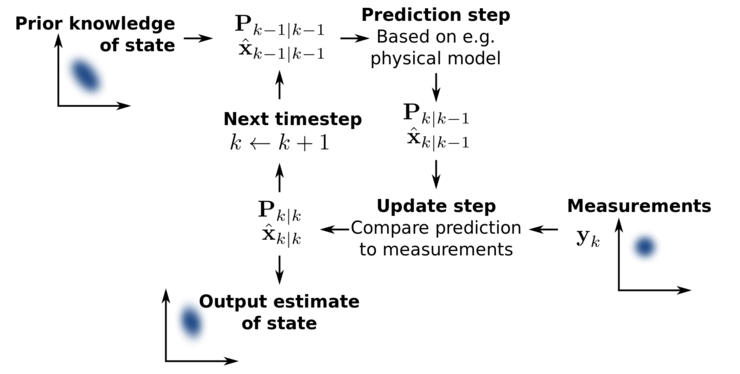
\includegraphics[width=\columnwidth]{pictures/chapter11/basic_concept_of_Kalman_filtering.png}
\caption{칼만 필터의 기본 컨셉}
\end{figure}

단, 칼만 필터는 선형 시스템에만 해당, 적용된다. 우리 로봇 및 센서는 대부분 비선형 시스템인 경우가 많은데 이를 위해 칼만 필터를 수정한 확장 칼만필터, EKF (Extended Kalman Filter) 가 널리 이용된다. 이 이외에도 EKF 의 정확성을 보완한 무향 칼만 필터, UKF (Unscented Kalman Filter), 속도를 개선한 Fast Kalman filter 등 많은 KF 변종이 있으며 지금도 많이 연구되고 있다. 또한, 파티클 필터와 함께 사용하는 RBPF (Rao-Blackwellized Particle Filter) 등 다른 알고리즘과 함께 사용되는 경우도 흔히 찾아 볼 수 있다.


\subsubsection{파티클 필터(Particle filter)}

파티클 필터(Particle Filter)는 물체 추적에 있어서 최근에 가장 많이 사용되고 있는 알고리즘이다. 그 대표적으로는 파티클 필터을 이용한 몬테카를로 위치추정 (Monte Carlo Localization) 가 있다. 이 전에 설명한 칼만 필터의 경우 선형 시스템과 가우시안 잡음(Gaussian Noise)가 있는 시스템의 경우에는 그 정확도가 보장되지만 그렇지 못한 경우에는 정확도가 보장되지 못하다는 문제가 있다. 우리 주변의 현실 세계의 문제는 대부분 비선형 시스템이라는 점이 문제가 된다.

로봇과 센서도 마찬가지이여서 위치 추정에 파티클 필터가 많이 사용된다. 칼만 필터가 대상체를 선형 시스템을 가정하고 선형 운동으로 파라미터를 찾아가는 해석적 방법이라고 한다면, 파티클 필터는 시행 착오(try-and-error)법을 기반으로한 시뮬레이션을 통하여 예측하는 기술으로 대상 시스템에 확률 분포로 임의로 생성된 추정값을 파티클(입자) 형태로 나타낸다고 하여서 파티클 필터라는 이름이 붙었다. 이는 SMC(Sequential Monte Carlo) 방법 또는 몬테카를로 방법이라고도 불리운다.

파티클 필터는 여타 위치 추정 알고리즘과 마찬가지로 연속적으로 들어오는 정보 중에 오차가 포함되어 있다고 가정하고 대상체의 위치를 추정하게 된다. SLAM 에서 사용할 때도 로봇의 오도메트리 값과 거리 센서를 이용한 환경 계측 값 등이 관측 값으로 사용되어 로봇의 현재 위치를 추정하게 된다. 

파티클 필터 방법에서는 위치 불확실성을 샘플이라 불리우는 파티클(입자)의 무리로 이를 묘사한다. 그 입자를 로봇의 운동 모델과 확률에 근거하여 새로운 추정 위치로 이동해 가며 실제 계측 값에 따라 각 입자에 가중치(weight)를 주면서 점점 정확한 위치로 잡음을 줄이며 추정해 나가는 과정을 거치게 된다. 여기서 각 파티클(입자)를 이용하게 되는데, $particle = pose(x,y,t), weight$ 와 같이 각 파티클은 로봇의 추정 위치를 나타내는 임의의 작은 입자로 로봇의 $x, y theta$ 좌표와 각 파티클의 가중치($weight$) 로 표현된다. 

이 파티클 필터는 아래의 5가지 과정을 거치며 1번 초기화를 제외하고 2번~5번은 반복적으로 수행하며 로봇의 위치 값을 추정하게 된다. 그 과정은 다음과 같다. 즉, X-Y 좌표 평면상에 로봇의 위치를 확률로 나태난 입자의 분포를 계측값을 기반으로 갱신해 나아가며 로봇의 위치를 추측하는 방식이다. 

자세한 파티클의 공식 관련은 로봇 공학에서 확률 관련 분야의 교과서로 불리우는 그 이름도 유명한 Sebastian Thrun\footnote{\url{http://robots.stanford.edu/}} (스탠포드 교수, 구글 펠로우, 유다시티 창업자)의 저서인 "Probabilistic Robotics"\cite{thrun2005probabilistic} 이라는 책이 있다. 필자는 로봇 공학을 공부하고 싶다는 사람이 있다면 이 책을 적극 추천하는 바이다. 그리고 우리 나라 Open Robotics 분야에서 많은 활동을 하고 계시는 KITECH의 양광웅 연구원님의 블로그와 카페,  로봇 공학 관련 블로그를 운영중이신 황병훈님의 파티클 필터관련 글도 도움이 될 것이다. 그리고 앞서 이야기한 "Probabilistic Robotics" 과 관련하여 유다시티의 강좌\footnote{\url{https://www.udacity.com/course/cs373}}가 있다는 것을 줄리앙님을 통해서 알게되었다. 필자도 꼭 수강하고 싶은 내용이 즐비하다. 관심 있는 사람은 "Artificial Intelligence for Robotics" 온라인 강좌를 참고하도록 하자.


\setcounter{num}{0}

\vspace{\baselineskip}
\noindent
\stepcounter{num}
\thenum) 초기화(initialization)\\
전역 위치 추정(Global localization)면에서 처음에는 로봇 위치 및 방향을 알 수 없기 때문에 N개의 입자 ($particle_i = pose(x_i,y_i,t_i)$) 를 임의로 뿌리게 된다. 이는 가장 처음에만 수행하는 것으로 입자의 가중치는 모두 같으며(1/N) 그 합은 1이 된다. 

\vspace{\baselineskip}
\noindent
\stepcounter{num}
\thenum) 예측(prediction)\\
로봇의 움직임을 기술한 시스템 모델(system model)에 기반하여 로봇의 이동량에 잡음(noise)을 포함하여 각 입자들을 이동시킨다.

\vspace{\baselineskip}
\noindent
\stepcounter{num}
\thenum) 보정(update)\\
계측된 센서 정보들을 기반으로 각 입자가 존재할 확률을 계산하고, 이를 반영하여 각 입자의 가중치가 1이 되도록 가중치의 값을 갱신한다. 이 갱신후의 입자 값은 초기화에서 주어졌던 $particle_i = pose(x_i,y_i,t_i)$, $weight_i (i=1,...,N)$ 이 예측과 갱신을 거쳐 새로운 상태가 된다. 

\vspace{\baselineskip}
\noindent
\stepcounter{num}
\thenum) 위치 추정(pose estimation)\\
N개의 모든 각 입자의 위치 $(x,y,t)$ 와 가중치 (weight)를 곱하여 로봇의 추정 위치를 계산한다.

\vspace{\baselineskip}
\noindent
\stepcounter{num}
\thenum) 재추출(Resampling)\\
새로운 입자를 생성하는 단계로 가중치가 작은 입자를 없애고 가중치가 높은 입자를 중심으로 기존의 입자의 특성인 입자의 위치정보를 물려받은 새로운 입자를 추가로 생성한다. 여기서 입자 수 N은 그대로 유지해야 한다.

추가로, 파티클 필터는 샘플의 개수가 충분하다면 칼만 필터의 개선한 EKF나 UKF보다 위치 추정이 정확하지만 그 개수가 충분하지 않으면 정확하지 않을 수 있다. 이러한 부분을 해결하기 위한 접근법으로 파티클 필터와 와 칼만 필터를 동시에 사용하는 방법인 RBPF (Rao-Blackwellized Particle Filter)\cite{grisetti2005improving}\cite{grisetti2007improved} 기반의 SLAM도 매우 일반적으로 사용되고 있다. 궁금하면 관련 자료를 찾아봐도 좋을 듯 싶다.


\subsubsection{Graph 및 Bundle adjustment 를 이용한 SLAM}

칼만 필터와 그 확장 개념들의 유사 칸만 필터 시리즈, 그리고 파티클 필터라고해서 모든 것에 만능은 아니다 예를들어, 무인 자동차와 같이 매우 넓은 미지의 구역을 SLAM 해야하는 경우에는 그 연산량이 매우 증가하게 되는데 이 경우 연상량으로 실시간성이 떨어지게 마련이다. 이러한 문제점을 보완하기 위해서 최근에는 목적에 따라서 그래프(Graph) 기반 SLAM 방법 및 Bundle adjustment\footnote{\url{http://en.wikipedia.org/wiki/Bundle_adjustment}} 방법이 많이 연구되고 있다. 그래프 기반 SLAM (GraphSLAM)의 경우에는 로봇과 계측한 데이터의 특징들의 위치 관계를 구속조건들로 정의하여 그래프를 작성하고, 그 그래프가 교차하는 지점에서 전체 그래프에 누적된 오차를 최소화하는 방법을 채택한 방법으로 1997년에 처음 F. Lu 와 E. Milios 에 의해 고안되어 광범위 SLAM 에서 많이 연구되고 있는 방법이다. 그리고, 카메라와 특징들의 위치를 동시에 보정하는 용도로 Bundle Adjustment 방법도 최근에 극 부상하고 있는 방법이다. 이 들의 방법에 대해서는 나중에 좀 더 자세히 다루어 보기로 한다.


%-------------------------------------------------------------------------------
\subsection{OpenSLAM과 Gmapping}

SLAM 분야는 앞서 설명하였듯이 로봇 공학에서 매우 많이 연구되고 있는 분야이다. 이러한 정보는 최신 학술지 및 학회 발표 자료를 통해 찾아 볼 수 있는데, 이 들의 연구 중 오픈소스로 공개된 부분이 상당히 많다. 이들의 정보는 OpenSLAM 이라는 그룹이 이를 모두 정리하였고, \url{OpenSLAM.org} 이라는 사이트에서 확인 할 수 있다. 우리가 꼭 방문해봐야 할 사이트라고 할 수 있다. 꼭 방문해 보길 바란다.

예를들어, 2D-I-SLSJF, CAS-Toolbox, CEKF-SLAM, DP-SLAM, EKFMonoSLAM, FLIRTLib, G2O, GMapping, GridSLAM, HOG-Man, iSAM, Linear SLAM, Max-Mixture, MTK, OpenRatSLAM, OpenSeqSLAM, ParallaxBA, Pkg. of T.Bailey, RGBDSlam, Robomap Studio, RobotVision, ro-slam, SLAM6D, SLOM, SSA2D, tinySLAM, TJTF for SLAM, TORO, TreeMap, vertigo 등 30여가지의 SLAM 소스와 관련 툴을 공개하고 있다.

우리가 전 강좌에서 사용한 gmapping\footnote{\url{http://www.openslam.org/gmapping.html}} 또한 이곳에 소개 되고 있고, ROS 커뮤니티에서는 이를 SLAM 에서 많이 사용하고 있다. gmapping 에 관련해서는 2가지 논문\cite{grisetti2005improving}\cite{grisetti2007improved}이 소개되고 있다. 하나는 ICRA 2005에서 발표된 것과 또 다른 하나는 2007년 Robotics, IEEE Transactions on 논문지에 발표된 논문이다.

이 논문들은 어떻게 하면 입자수를 최소한으로 줄여서 연산량을 줄이고 실시간성을 낼 수 있을까에 대한 논문으로 주요 접근 방법으로는 위에서 설명한 Rao-Blackwellized particle filter 를 사용하였다. 자세한 사항은 논문을 참조하기 바라며, 개략적인 설명은 위 파티클 필터의 설명으로 이해할 수 있을 것이다.

이것으로 SLAM 강좌를 마쳤다. gmapping 에 대한 설명은 파티클 필터 설명으로 대체하였으니 더 자세한 설명은 논문을 참고하라는 말을 하고 싶다. 이 강좌에서 자세한 논문 리뷰까지는 할 수 없을테니 말이다. 다음 강좌에서는 내비게이션으로 넘어가도록 하겠다.

\newpage
%-------------------------------------------------------------------------------
\section{내비게이션 실습편}\index{내비게이션 실습편}
\label{sec:NavigationExe}

%-------------------------------------------------------------------------------
\subsection{Navigation 따라하기}

내비게이션(Navigatoin)에 대한 설명에 앞서서 거북이를 이용하여 내비게이션 하는 방법에 대해 설명하고 넘어가도록 하겠다. 내비게이션 에 대한 이론 강좌는 SLAM 강좌때와 같은 순서대로 내비게이션 응용편, 이론편 강좌로 추후 이어지는 강좌에서 이어서 설명하도록 하겠다.

%-------------------------------------------------------------------------------
\subsection{내비게이션을 위한 로봇 하드웨어}

내비게이션을 위한 로봇 하드웨어는 \textbf{섹션~\ref{subsubsec:kobuki_robot_sensor}~\nameref{subsubsec:kobuki_robot_sensor}(pp.\pageref{subsubsec:kobuki_robot_sensor})} 에서 이미 언급한 사항과 동일하다. 모바일 로봇으로는 거북이를 이용하고 센서로는 LRF를 를 사용하였다. 계측 환경도 SLAM 떄와 마찬가지이다. 자세한 내용은 \textbf{섹션~\ref{sec:SlamExe}~\nameref{sec:SlamExe}(pp.\pageref{sec:SlamExe})}을 참고하도록 하자. 그리고, 이번 강좌에서는 이전 SLAM 에서 작성한 \textbf{지도}를 이용하여 정해진 목적지까지 로봇을 이동시키는 내비게이션에 대해서 알아보도록 하자.

%-------------------------------------------------------------------------------
\subsection{내비게이션을 위한 ROS 패키지}

본 강좌에서 사용할 내비게이션 관련 ROS 패키지는 kobuki 메타 패키지와 이전 SLAM 강좌에서 작성한 kobuki\_tf 패키지 , navigation 메타 패키지의 move\_base, amcl, map\_server 패키지 등이 이다. 아래와 같이 미리 모두 설치해 두도록 하자. 본 강좌는 따라하기 강좌이기에 때문에 실행 방법만을 기술할 예정이다. 각 패키지의 설명은 다음 강좌에서 매우 자세히 다루도록 하겠다. 

※ 이번 강좌 부터는 작업 혼란을 막기 위하여, 모든 패키지를 거북이에 설치하고 진행하도록 하겠다. 패키지의 설치, 각 노드, 런치파일의 실행은 모두 거북이 본체와 연결된 랩톱에서 실행해야 한다. 단, RViz 및 기타 시각화 관련해서는 데스크톱에서 실행해도 무방하다.

\vspace{\baselineskip}
\begin{lstlisting}[language=ROS]
$ sudo apt-get install ros-indigo-kobuki*
$ sudo apt-get install ros-indigo-navigation
\end{lstlisting}

센서 패키지로는 사용하는 센서에 맞도록 관련 패키지를 아래와 같이 설치하도록 하자. 이번 강좌에서는 1) LRF 를 이용하여 설명하도록 하고 다른 센서에 대해서는 별도로 다루도록 하겠다.

\setcounter{num}{0}

\vspace{\baselineskip}
\noindent
\stepcounter{num}
\thenum) Hokuyo LRF\footnote{\url{https://www.hokuyo-aut.jp/02sensor/07scanner/utm_30lx.html}} (URG-04LX 및 UTM-30LX 시리즈)

\begin{lstlisting}[language=ROS]
$ sudo apt-get install ros-indigo-urg-node
\end{lstlisting}
 
\noindent
\stepcounter{num}
\thenum) Kinect

\begin{lstlisting}[language=ROS]
$ sudo apt-get install ros-indigo-openni-camera ros-indigo-openni-launch
\end{lstlisting}

\noindent
\stepcounter{num}
\thenum) Xtion

\begin{lstlisting}[language=ROS]
$ sudo apt-get install ros-indigo-openni2-camera ros-indigo-openni2-launch
\end{lstlisting}


%-------------------------------------------------------------------------------
\subsection{내비게이션 실행}

\setcounter{num}{0}

\vspace{\baselineskip}
\noindent
\stepcounter{num}
\thenum) 소스 다운로드 및 컴파일\\
우선, 오로카 Github 주소에서 관련 패키지를 다운로드 받는다. 그 후, 컴파일을 해준다.

\vspace{\baselineskip}
\begin{lstlisting}[language=ROS]
$ cd ~/catkin_ws/src
$ git clone https://github.com/oroca/oroca-ros-pkg.git
$ cd ~/catkin_ws && catkin_make
\end{lstlisting}

\vspace{\baselineskip}
\noindent
\stepcounter{num}
\thenum) 거북이 노드 실행\\
roscore 를 실행한 후, 거북이 노드를 실행한다.

\vspace{\baselineskip}
\begin{lstlisting}[language=ROS]
$ roscore
$ roslaunch kobuki_node minimal.launch --screen
\end{lstlisting}

\vspace{\baselineskip}
\noindent
\stepcounter{num}
\thenum) kobuki\_navigation 실행\\
kobuki\_navigation 패키지는 복수의 런치 파일로 구성되어 있다. 아래의 런치 파일을 실행하게 되면 LRF의 드라이버인 urg\_node 노드, 좌표 변환을 위한 tf 를 활용한 kobuki\_tf 노드, kobuki 3차원 모델 정보, 이전 작성해둔 지도를 불러오는 map\_server 노드, AMCL(Adaptive Monte Carlo Localization) 노드, move\_base 노드가 함께 실행된다.

\vspace{\baselineskip}
\begin{lstlisting}[language=ROS]
$ sudo chmod a+rw /dev/ttyACM0
$ roslaunch kobuki_navigation kobuki_navigation.launch
\end{lstlisting}

아래의 내용은 kobuki\_navigation.launch 의 각 설정 값이다. 사용하는 로봇, 센서에 따라 많은 설정값이 있다. 우선, 필자는 이전에 SLAM 강좌에서 다루었던 거북이 로봇과 LRF 를 이용하여 설정하여 보았다. 추후에 이 런치 파일을 각자 로봇에 적용하는 방법도 별도의 강좌를 통해서 설명하도록 하겠다.

\vspace{\baselineskip}
\begin{lstlisting}[language=XML]
<launch>
  <!-- kobuki model -->
  <arg name="urdf_file" 
    default="$(find xacro)/xacro.py '$(find kobuki_description)/urdf/kobuki_standalone.urdf.xacro'" />
  <param name="robot_description" command="$(arg urdf_file)" />
  <node pkg="robot_state_publisher" type="robot_state_publisher" name="robot_state_publisher" output="screen">
    <param name="publish_frequency" type="double" value="5.0" />
  </node>

  <!-- sensor -->
  <node pkg="urg_node" type="urg_node" name="kobuki_urg_node" output="screen">
    <param name="frame_id" value="base_scan" />
  </node>

  <!-- tf -->
  <node pkg="kobuki_tf" type="kobuki_tf" name="kobuki_tf" output="screen">
  </node>

  <!-- Map server -->
  <arg name="map_file" default="$(find kobuki_navigation)/maps/map.yaml"/>
  <node name="map_server" pkg="map_server" type="map_server" args="$(arg map_file)">
  </node>

  <!-- AMCL -->
  <include file="$(find kobuki_navigation)/launch/amcl.launch.xml"/>

  <!-- move_base -->  
  <arg name="cmd_vel_topic" default="/mobile_base/commands/velocity" />
  <arg name="odom_topic" default="odom" />
  <node pkg="move_base" type="move_base" respawn="false" name="move_base" output="screen">
    <rosparam file="$(find kobuki_navigation)/param/costmap_common_params.yaml" command="load" ns="global_costmap" />
    <rosparam file="$(find kobuki_navigation)/param/costmap_common_params.yaml" command="load" ns="local_costmap" />
    <rosparam file="$(find kobuki_navigation)/param/local_costmap_params.yaml" command="load" />
    <rosparam file="$(find kobuki_navigation)/param/global_costmap_params.yaml" command="load" />
    <rosparam file="$(find kobuki_navigation)/param/base_local_planner_params.yaml" command="load" />
    <rosparam file="$(find kobuki_navigation)/param/move_base_params.yaml" command="load" />
    <remap from="cmd_vel" to="$(arg cmd_vel_topic)"/>
    <remap from="odom" to="$(arg odom_topic)"/>
  </node>

</launch>
\end{lstlisting}

\vspace{\baselineskip}
\noindent
\stepcounter{num}
\thenum) RViz 실행\\

내비게이션에서 목적지 지정 명령 및 그 결과를 눈으로 확인 할 수 있도록 ROS 의 시각화툴인 RViz를 구동하도록 하자. 구동 시에 아래와 같이 옵션을 붙여주면 디스플레이 플러그인들이 처음부터 추가되어 매우 편리하다.

\vspace{\baselineskip}
\begin{lstlisting}[language=ROS]
$ rosrun rviz rviz -d `rospack find kobuki_navigation`/rviz/kobuki_nav.rviz
\end{lstlisting}

이를 실행시켜주면 아래와 같은 화면을 볼 수 있을 것이다. 우측 지도에 녹색 화살표가 잔뜩 보일텐데 이는 SLAM 이론편 강좌에서 설명하였던 파티클 필터의 각 입자들이다. 나중에 다시 설명하겠지만 내비게이션 또한 파티클 필터를 이용하기 때문이다. 그 녹색 화살표의 가운데 쯤에 있는 것이 거북이 로봇임을 확인 할 수 있을 것이다.

\begin{figure}[h]
\centering
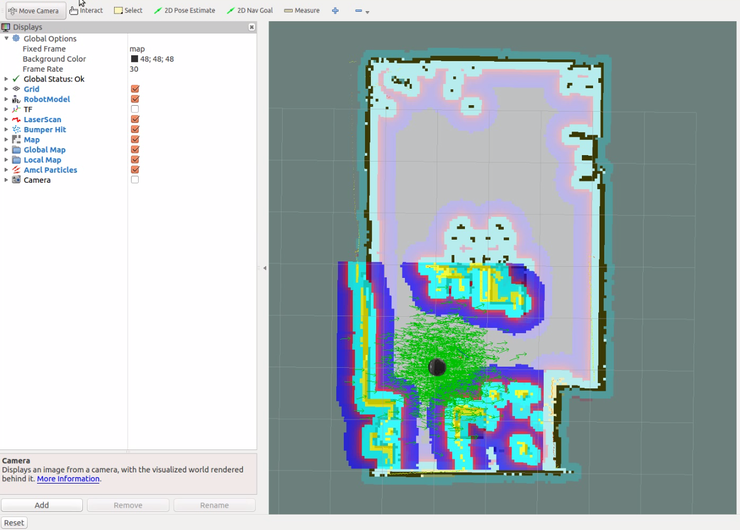
\includegraphics[width=0.9\columnwidth]{pictures/chapter11/navigation_rviz.png}
\caption{RViz에서 확인 가능한 파티클(로봇 주위의 녹색 화살표)}
\end{figure}

\vspace{\baselineskip}
\noindent
\stepcounter{num}
\thenum) 초기 위치 추정\\
제일 먼저 로봇의 초기 위치 추정 작업을 거쳐야 한다. RViz 의 상단의 메뉴바 중에 "2D Pose Estimate" 를 누르면 매우 큰 녹색 화살표가 나타날 것이다. 이를 대략적으로 로봇 중앙에 위치하여 클릭하고, 마우스 버튼을 놓치 않은 상태로 로봇이 정면 방향을 가르키도록 녹색 화살표를 드래그 한다. 이 것은 초기에 대략 적인 로봇의 위치를 추정하기 위한 일종의 명령어이다. 이 과정을 거치면 로봇은 지정된 위치$(x,y)$ 와 방향$(θ)$ 를 가지고 스스로 자신의 위치를 추정하여$(x, y, θ)$ 셋팅 될 것이다. 글로 표현하기 어려우니 아래에 첨부한 동영상의 처음 부분을 참고하도록 하자.

\vspace{\baselineskip}
\noindent
\stepcounter{num}
\thenum) 목적지 설정 및 로봇 이동\\
모든 준비가 완료되었으면 내비게이션 명령을 내려보자. RViz 의 상단의 메뉴바 중에 "2D Nav Goal" 를 누르면 마찬가지로 매우 큰 녹색 화살표가 나타날 것이다. 이를 로봇을 이동시키고자 하는 위치에 클릭하고, 드래그 하여 방향도 설정해주도록 하자. 그러면 로봇은 작성된 지도를 기반으로 목적지까지 장애물을 피하여 이동할 것이다. 이는 아래의 동영상으로 설명을 대체 하기로 한다.

다음 강좌에서는 위에서 실행했던 패키지들의 자세한 소스 설명 및 설정법에 대해서 추가 설명을 하도록 하자. SLAM 강좌와 비슷한 방식으로 실습편, 응용편, 이론편 강좌로 나누어 진행할 예정이다.

\begin{figure}[h]
\centering
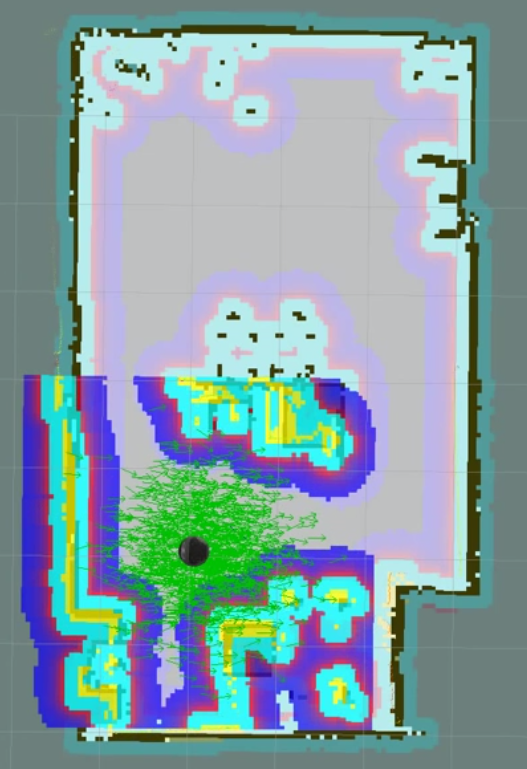
\includegraphics[width=0.24\columnwidth]{pictures/chapter11/navigation_test1.png}
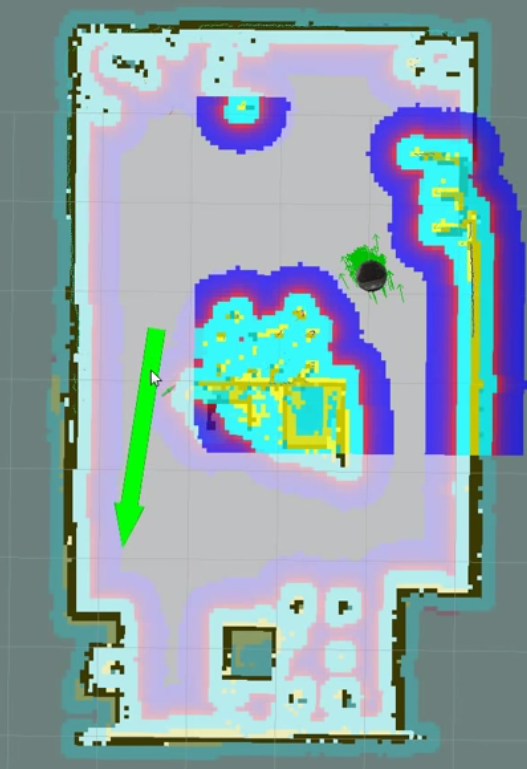
\includegraphics[width=0.24\columnwidth]{pictures/chapter11/navigation_test3.png}
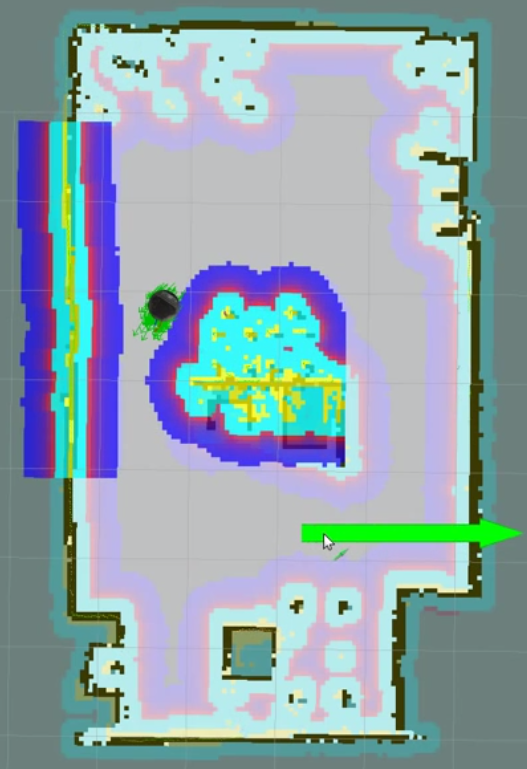
\includegraphics[width=0.24\columnwidth]{pictures/chapter11/navigation_test4.png}
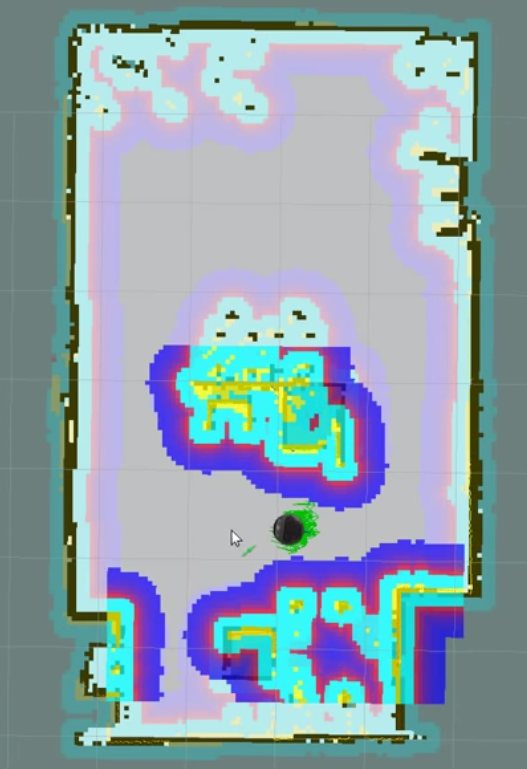
\includegraphics[width=0.24\columnwidth]{pictures/chapter11/navigation_test5.png}
\caption{목적지 설정(큰 화살표) 및 로봇이 이동해 가는 모습}
\end{figure}

% \begin{figure}[h]
% \centering
% 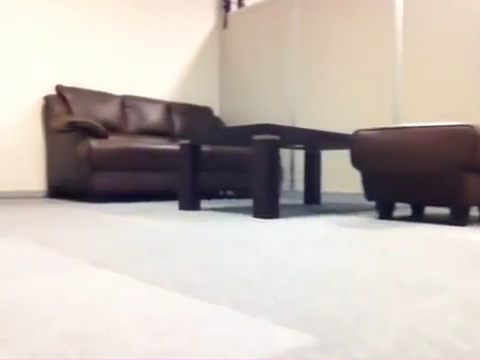
\includegraphics[width=0.5\columnwidth]{pictures/chapter11/navigation_camera.png}
% \caption{로봇 장착된 카메라로 촬영된 내비게이션 동작 화면}
% \end{figure}

\newpage
%-------------------------------------------------------------------------------
\section{내비게이션 응용편}\index{내비게이션 응용편}
\label{sec:NavigationApp}

섹션~\ref{sec:NavigationExe}~\nameref{sec:NavigationExe}(pp.\pageref{sec:NavigationExe})이 단순히 따라해보는 강좌였다면 이번 강좌에서는 내비게이션(navigation) 에서 사용되는 ROS 패키지를 자세히 살펴보고 어떻게 작성, 설정하는지에 대해서 알아 보는 응용편이라고 할 수 있다. 즉, kobuki 메타 패키지와 LRF의 드라이버인 urg\_node 노드, 좌표 변환을 위한 tf 를 활용한 kobuki\_tf 노드, kobuki 3차원 모델 정보(kobuki\_description), 이전 작성해둔 지도를 불러오는 map\_server 노드, AMCL(Adaptive Monte Carlo Localization) 노드, move\_base 노드 에 대해 살펴볼 예정이다. 이는 앞서 진행한 섹션~\ref{sec:NavigationExe}~\nameref{sec:NavigationExe}(pp.\pageref{sec:NavigationExe})을 자신의 로봇에 적용해 볼 수 있는 응용편이라고 볼 수 있다. 내비게이션(navigation) 자체에 대한 이론적인 설명은 섹션~\ref{sec:NavigationTheory}~\nameref{sec:NavigationTheory}(pp.\pageref{sec:NavigationTheory}) 에서 설명하도록 하겠다.

이 과정에서 본 강좌는 거북이라는 플랫폼과 LRF 센서를 기반으로 설명하겠지만, 이를 응용하면 특정 로봇 플랫폼, 특정 센서에 국한되지 않고 자신만의 로봇으로 내비게이션 이 가능하게 될 것이다. 자신만의 로봇 플랫폼을 만들거나 거북이 로봇 플랫폼 위에 자신만의 스타일로 새로운 로봇을 구성하고 싶다면 이 강좌가 도움이 될 것이다.

%-------------------------------------------------------------------------------
\subsection{내비게이션}

내비게이션은 주어진 환경에서 현재 로봇의 위치로부터 지정한 목적지까지 이동하는 것이다. 이를 위해서는 주어진 환경의 가구, 물체, 벽 등의 기하학적인 정보 (geometry, geo-:토지, metry:측정)가 담긴 지도가 필요한데 이 부분에 대해서는 이전  SLAM 강좌에서 설명하였듯이 로봇이 자신의 위치 정보와 센서로부터 얻은 거리 정보로 지도를 얻을 수 있었다. 

\begin{figure}[h]
\centering
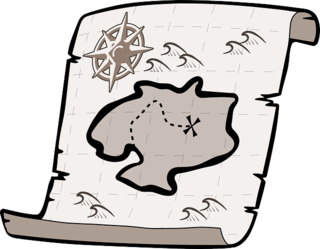
\includegraphics[width=0.5\columnwidth]{pictures/chapter11/treasure_map.png}
\caption{지도 (출처:pixabay.com, 라이선스:CC0)}
\end{figure}

내비게이션은 이 지도와 로봇의 엔코터, 관성 센서, 거리 센서 등을 이용하여 현재 위치로부터 지도상에 지정된 목적지 까지 이동하게 된다. 그 순서로는 아래와 같다.

\subsubsection{센싱 (sensing)}
지도상에서 로봇은 엔코더와 관성 센서(IMU 센서) 등으로 자신의 오도메트리(odometry) 정보 갱신하면서 거리 센서가 장착된 위치로부터 장애물(벽,물체,가구 등)과의 거리를 계측한다. 

\subsubsection{위치 추정 (localization / pose estimation)}
엔코더로부터의 바퀴 회전량, 관성 센서로부터의 관성 정보, 거리 센서로부터 장애물과의 거리 정보 등을 기반으로 기존에 작성해둔 지도상에 현재 로봇이 어디에 있는지 위치 추정(localization / pose estimation)하게 된다. 이때에 사용되는 위치 추정 방법론은 종류가 매우 많은데, 본 강좌에서는 파티클 필터 위치 추정 (particle filter localization) 이라고도 불리우는 Monte Carlo Localization (MCL) 의 변형인 AMCL (Adaptive Monte Carlo Localization)\cite{thrun2005probabilistic} 를 이용할 예정이다.

\subsubsection{모션 계획 (motion planning)}
이동 경로 계획 (path plannig)이라고도 불리우는 것으로, 그 현재 위치로부터 지도상에 지정받은 목표 지점까지 이동 궤적(trajectory)을 생성한다. 지도 전체상의 전역 이동 경로 계획(global path plannig)과 로봇 중심으로 일정 일부 지역을 대상으로 한 국부 이동 경로 계획(local path plannig) 으로 나누어 로봇의 이동 경로를 만든다. 우리는 장애물 회피 알고리즘인 Dynamic Window Approach\footnote{\url{http://en.wikipedia.org/wiki/Dynamic_window_approach}} (DWA) 를 기반으로 한 ROS의 move\_base 와 nav\_core 등의 이동 경로 계획 패키지를 이용할 예정이다.

\subsubsection{이동 / 장애물 회피 (move / collision avoidance)}
모션 계획에서 작성된 이동 궤적을 따라서 로봇에 속도 명령을 내려주면 로봇은 그 이동 궤적에 따라 목적지 까지 이동하게 된다. 이 이동 중에도 1번~3번의 센싱, 위치 추정, 모션 계획은 계속 수행 중이기이 때문에 갑자기 나타난 장애물, 이동 물체등은 Dynamic Window Approach (DWA) 알고리즘을 사용하여 회피하며 이동하게 된다.

%-------------------------------------------------------------------------------
\subsection{내비게이션에 필요한 정보}

\begin{figure}[h]
\centering
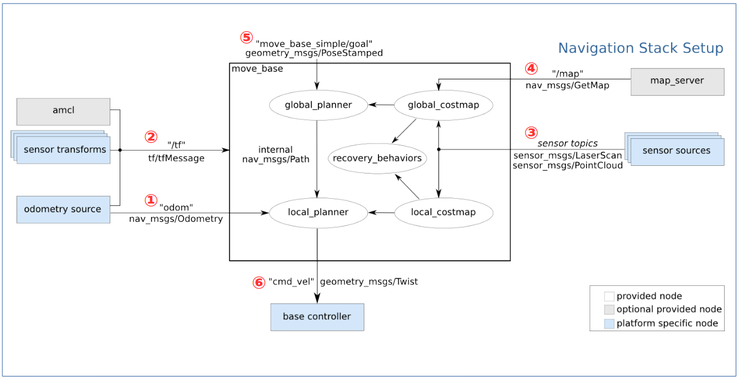
\includegraphics[width=\columnwidth]{pictures/chapter11/navigation_full_flow.png}
\caption{내비게이션 스택 설정에 관한 각 필수 노드와 토픽 관계도 (출처: http://wiki.ros.org/navigation/Tutorials/RobotSetup CC-BY 3.0 )}
\end{figure}

위 그림은 ROS의 내비게이션 패키지 구동에 필요한 필수 노드와 토픽들의 관계도를 설명한 그림이다. 이를 내비게이션에 필요한 정보(토픽)를 중심으로 설명하도록 하겠다.

\subsubsection{오도메트리 ( "odom", nav\_msgs/Odometry )}
로봇의 오도메트리 정보는 국부 이동 경로 계획(local path planning) 에서 사용하게 되는데 로봇의 현재 속도 등의 정보를 받아서 국부 이동 경로를 생성하거나 장애물 회피 등에 사용된다.

\subsubsection{상대 위치 변환 ( "/tf", tf/tfMessage )}
로봇의 센서의 위치를 예를들어 base\_scan 라고 할 때, 이 센서 위치는 로봇의 하드웨어적 구성에 따라 위치가 상대적으로 바뀌기 때문에 ROS에서는 tf 라는 상대 위치 변환을 이용한다. 이는 단순히 오도메트리로 로봇의 위치를 알게되는데 "그 로봇의 위치로부터 x,y,z 좌표 상 센서가 얼마만큼 떨어져 있다." 라는 형태로 기술해 주는 것이다. 예를들어,  odom → base\_linkfootprint → base\_link → base\_scan 의 변환을 거쳐서 토픽으로 발행하게 된다. 이는 move\_base 노드에서 이 정보를 받아 로봇의 위치와 센서의 위치를 가지고 이동 경로 계획을 수행하게 된다.

\subsubsection{거리 센서 ( sensor topics, sensor\_msgs/LaserScan or sensor\_msgs/PointCloud  )}
센서로부터 측정된 거리 값을 의미한다. 흔히, LRF 및 Kinect, Xtion 등이 사용된다. 이 거리 센서는 로봇 위치 추정 방법인 AMCL(adaptive Monte Carlo localization) 을 이용하여 로봇의 현재 위치 추정, 로봇의 모션 계획에 사용된다. 우리는 이 센서 값을 "scan" 이라는 토픽 명으로 방행할 예정이다.

\subsubsection{지도 ( "/map", nav\_msgs/GetMap )}
내비게이션에서는 점유 격자 지도(occupancy grid map) 를 사용하게 된다. 이 강좌에서는 이 전에 작성해둔 "map.pgm" 과 "map.yaml" 을 map\_server 패키지를 이용하여 발행할 것이다. 

\subsubsection{목표 좌표 ( "move\_base\_simple/goal", geometry\_msgs/PoseStamped )}
목표 좌표는 유저가 직접 명령하게 된다. 이는 태블릿과 같은 장비로 별도의 목표 좌표 명령 패키지를 작성하여 사용하는 것도 가능하나, 이번 강좌에서는 ROS 의 시각화 툴인 RViz 에서 목표 좌표를 지정할 예정이다. 목표 좌표는 2차원 상에 x, y, θ 으로 구성되어 있다.

\subsubsection{속도 명령 ( "cmd\_vel", geometry\_msgs/Twist )}
최종적으로 계획된 이동 궤적에 따라 로봇을 움직이는 속도 명령을 발행하는 것으로 로봇은 목적지까지 이동하게 된다. 우리는 이 속도 명령을 "/mobile\_base/commands/velocity" 라는 토픽명으로 발행할 예정이다.


%-------------------------------------------------------------------------------
\subsection{kobuki\_navigation 의 각 노드 및 토픽 상태}

\vspace{\baselineskip}
\begin{lstlisting}[language=ROS]
$ roslaunch kobuki_node minimal.launch --screen
$ roslaunch kobuki_navigation kobuki_navigation.launch
\end{lstlisting}

\noindent
\textbf{섹션~\ref{sec:NavigationExe}~\nameref{sec:NavigationExe}(pp.\pageref{sec:NavigationExe})}에서 설명했던 것처럼 위와 같이 kobuki\_node 와 kobuki\_navigation 를 실행하게 되면 내비게이션에 필요한 조건을 갖추게 된다. 

\vspace{\baselineskip}
\begin{lstlisting}[language=ROS]
$ rqt_graph
\end{lstlisting}

이 상태에서 위와 같이 ROS 환경에서 실행 중인 노드와 토픽 정보를 확인할 수 있는 rqt\_graph 를 실행해주면 아래와 같이 그 정보들이 시각화되어 확인해 볼 수 있다. 아래의 다이어그램을 보면 알 수 있듯이, 위에서 설명한 내비게이션에 필요한 정보는 각각 /odom, /tf,  /scan, /map, /mobile\_base/commands/velocity 이라는 토픽명으로 발행/구독되고 있으며, move\_base\_simple/goal 는 ROS 의 시각화 툴인 RViz 에서 목표 좌표를 지정할 경우에 발행되게 되어 있다.

\begin{figure}[h]
\centering
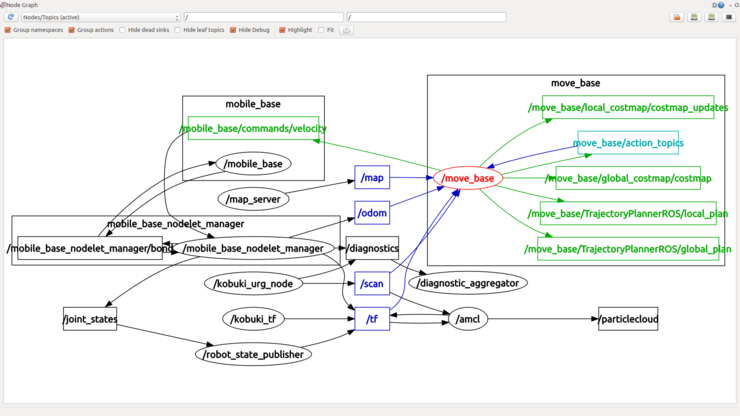
\includegraphics[width=\columnwidth]{pictures/chapter11/navigation_qt_graph.png}
\caption{kobuki\_navigation 의 각 노드 및 토픽 상태}
\end{figure}

%-------------------------------------------------------------------------------
\subsection{kobuki\_navigation 패키지}

\subsubsection{패키지 생성}

\vspace{\baselineskip}
\begin{lstlisting}[language=ROS]
$ cd ~/catkin_ws/src/
$ catkin_create_pkg kobuki_navigation amcl move_base kobuki_node kobuki_tf urg_node map_server
$ mkdir ./kobuki_navigation/launch ./kobuki_navigation/maps ./kobuki_navigation/param ./kobuki_navigation/rviz
\end{lstlisting}

위의 명령어로 kobuki\_navigation 이라는 내비게이션 패키지가 생성되었다. 뒤에 이어진 옵션으로 amcl move\_base kobuki\_node kobuki\_tf urg\_node map\_server 가 붙는데 이는 이 패키지가 의존하는 기존 패키지들을 의미한다. 

그리고, 이 패키지안에 런치 파일을 넣는 launch 폴더, 작성된 지도를 저장하는 maps폴더, 각 종 파라미터 정보를 담는 param 폴더, ROS 시각화 툴인 RViz의 설정 정보 파일을 넣는 rviz 폴더를 생성하였다. 이번 패키지에는 기존 패키지들의 설정만으로 구성되는 패키지이기에 실질적으로 컴파일 해야 할 소스파일이 없기에 src 폴더는 생략하기로 한다.

관련 소스는 \url{https://github.com/oroca/oroca-ros-pkg} 에서 공개하고 있다. 필요한 경우에는 참고하길 바란다.

\subsubsection{구성 파일}

내비게이션을 위해서는 아래와 같이 내비게이션 노드와 관련된 패키지들을 구동하는 launch, xml 파일, 각 종 파라미터 설정을 하는 yaml 파일, 지도 관련 파일, rviz 설정 파일이 필요하다.

\vspace{\baselineskip}
\begin{lstlisting}[language=ROS]
/launch/kobuki_navigation.launch
\end{lstlisting}

거북이를 모바일 로봇으로 이용할 경우, kobuki\_navigation.launch 파일 하나로 모든 내비게이션 관련 패키지가 실행된다. 

\vspace{\baselineskip}
\begin{lstlisting}[language=ROS]
/launch/amcl.launch.xml
\end{lstlisting}

amcl.launch.xml 는 AMCL(Adaptive Monte Carlo Localization) 의 각 종 파라미터 설정 값을 담은 파일로 kobuki\_navigationl.launch 와 함께 사용된다.

\vspace{\baselineskip}
\begin{lstlisting}[language=ROS]
/param/move_base_params.yaml
\end{lstlisting}

모션 계획을 총괄적으로 담당하는 move\_base의 파라미터 설정 파일이다.

\vspace{\baselineskip}
\begin{lstlisting}[language=ROS]
/param/costmap_common_params.yaml
/param/global_costmap_params.yaml
/param/local_costmap_params.yaml
\end{lstlisting}

내비게이션에서는 점유 격자 지도(occupancy grid map) 를 사용하게 된다. 이 점유 격자 지도를 기반으로, 로봇의 위치와 센서로 부터 얻은 주변 정보를 이용하여 각 픽셀을 장애물/이동불가영역/이동가능영역 으로 계산하게 되는데 이때에 사용되는 개념이 costmap\footnote{\url{http://wiki.ros.org/costmap_2d}} 이다. 이 costmap 의 설정 파라미터이 위와 같은 같은데, 공통의 costmap\_common\_params.yaml 파일와 전역 영역 모션 플래밍에 필요한 global\_costmap\_params.yaml, 국부 영역에 필요한 local\_costmap\_params.yaml 으로 구성되어 있다.

\vspace{\baselineskip}
\begin{lstlisting}[language=ROS]
/param/base_local_planner_params.yaml
\end{lstlisting}

base\_local\_planner 는 최종적으로 로봇에게 이동 속도 명령을 넘겨주는 패키지로 이에 대한 설정 파라미터를 설정하는 파일이다.

\vspace{\baselineskip}
\begin{lstlisting}[language=ROS]
/maps/map.pgm
/maps/map.yaml
\end{lstlisting}

이전에 작성한 점유 격자 지도(occupancy grid map) 를 /maps 폴더에 저장하여 사용한다.

\vspace{\baselineskip}
\begin{lstlisting}[language=ROS]
/rviz/kobuki_nav.rviz
\end{lstlisting}

ROS 시각화 툴인 RViz의 설정 정보 파일 담은 파일이다. RViz 의 디스플레이 플러그인 중, Grid, RobotModel, TF, LaserScan, Bumper Hit, Map, Global Map, Local Map, Amcl Particles 을 불러오게 된다.

%-------------------------------------------------------------------------------
\subsection{kobuki\_navigation 설정}

거북이를 모바일 로봇으로 이용할 경우, kobuki\_navigation.launch 파일 하나로 모든 내비게이션 관련 패키지가 실행된다. 

\vspace{\baselineskip}
\begin{lstlisting}[language=ROS]
/launch/kobuki_navigation.launch
\end{lstlisting}

\vspace{\baselineskip}
\begin{lstlisting}[language=XML]
<launch>
  <!-- kobuki model -->
  <arg name="urdf_file" 
    default="$(find xacro)/xacro.py '$(find kobuki_description)/urdf/kobuki_standalone.urdf.xacro'" />
  <param name="robot_description" command="$(arg urdf_file)" />
  <node pkg="robot_state_publisher" type="robot_state_publisher" name="robot_state_publisher" output="screen">
    <param name="publish_frequency" type="double" value="5.0" />
  </node>

  <!-- sensor -->
  <node pkg="urg_node" type="urg_node" name="kobuki_urg_node" output="screen">
    <param name="frame_id" value="base_scan" />
  </node>

  <!-- tf -->
  <node pkg="kobuki_tf" type="kobuki_tf" name="kobuki_tf" output="screen">
  </node>

  <!-- Map server -->
  <arg name="map_file" default="$(find kobuki_navigation)/maps/map.yaml"/>
  <node name="map_server" pkg="map_server" type="map_server" args="$(arg map_file)">
  </node>

  <!-- AMCL -->
  <include file="$(find kobuki_navigation)/launch/amcl.launch.xml"/>

  <!-- move_base -->  
  <arg name="cmd_vel_topic" default="/mobile_base/commands/velocity" />
  <arg name="odom_topic" default="odom" />
  <node pkg="move_base" type="move_base" respawn="false" name="move_base" output="screen">
    <rosparam file="$(find kobuki_navigation)/param/costmap_common_params.yaml" 
                       command="load" ns="global_costmap" />
    <rosparam file="$(find kobuki_navigation)/param/costmap_common_params.yaml"
                       command="load" ns="local_costmap" />
    <rosparam file="$(find kobuki_navigation)/param/local_costmap_params.yaml" command="load" />
    <rosparam file="$(find kobuki_navigation)/param/global_costmap_params.yaml" command="load" />
    <rosparam file="$(find kobuki_navigation)/param/base_local_planner_params.yaml" command="load" />
    <rosparam file="$(find kobuki_navigation)/param/move_base_params.yaml" command="load" />
    <remap from="cmd_vel" to="$(arg cmd_vel_topic)"/>
    <remap from="odom" to="$(arg odom_topic)"/>
  </node>

</launch>
\end{lstlisting}

\subsubsection{거북이 3차원 모델 ( kobuki model )}
이 부분의 경우, kobuki\_description 패키지에서 kobuki\_standalone.urdf 의 로봇 3D 모델을 불러오고, robot\_state\_publisher 를 통해 조인트 정보와 같은 로봇 상태를 상대 위치 변환인 tf로 발행하게 된다. 이 과정이 있기에 RViz 에서 로봇의 3차원 모델을 볼 수 있게된다.

\vspace{\baselineskip}
\begin{lstlisting}[language=XML]
<arg name="urdf_file" 
        default="$(find xacro)/xacro.py '$(find kobuki_description)/urdf/kobuki_standalone.urdf.xacro'" />
<param name="robot_description" command="$(arg urdf_file)" />
<node pkg="robot_state_publisher" type="robot_state_publisher" 
           name="robot_state_publisher" output="screen">
  <param name="publish_frequency" type="double" value="5.0" />
</node>
\end{lstlisting}

\subsubsection{센서 ( sensor )}
아래의 내용은 거북이에 장착되어 있는 LRF 를 구동하기 위한 구문으로 "frame\_id" 파라미터를 "base\_scan" 으로 변환시켜 실행시키도록 한다.

\vspace{\baselineskip}
\begin{lstlisting}[language=XML]
<node pkg="urg_node" type="urg_node" name="kobuki_urg_node" output="screen">
  <param name="frame_id" value="base_scan" />
</node>
\end{lstlisting}

\subsubsection{상대 위치 변환 ( tf )}
오도메트리부터 센서 위치까지의 상대 위치 변환 (odom → base\_footprint → base\_link → base\_scan) 정보를 tf 형태로 발행하는 kobuki\_tf 를 함께 실행하게 된다.

\vspace{\baselineskip}
\begin{lstlisting}[language=XML]
<node pkg="kobuki_tf" type="kobuki_tf" name="kobuki_tf" output="screen">
</node>
\end{lstlisting}

\subsubsection{지도 서버 ( Map server )}
kobuki\_navigation/maps/ 폴더에 저장된 지도 정보(map.yaml)를 불러와 map\_server 노드에 의해 토픽 형태로 지도가 발행된다.

\vspace{\baselineskip}
\begin{lstlisting}[language=XML]
<arg name="map_file" default="$(find kobuki_navigation)/maps/map.yaml"/>
<node name="map_server" pkg="map_server" type="map_server" args="$(arg map_file)">
</node>
\end{lstlisting}

\subsubsection{AMCL (Adaptive Monte Carlo Localization)}
AMCL관련하여 amcl 노드를 실행시키며, 관련 파라미터를 설정한다.

\vspace{\baselineskip}
\begin{lstlisting}[language=XML]
<include file="$(find kobuki_navigation)/launch/amcl.launch.xml"/>
\end{lstlisting}

\subsubsection{move\_base}
모션 계획에 필요한 costmap 관련 파라미터와 로봇에게 이동 속도 명령을 넘겨주는 base\_local\_planner 에 대한 설정 파라미터, 모션 계획을 총괄적으로 담당하는 move\_base의 파라미터를 설정한다. 더 자세한 설명은 아래 "kobuki\_navigation 관련 세부 파라미터 설정"에서 더 자세히 다루도록 하겠다.

\vspace{\baselineskip}
\begin{lstlisting}[language=XML]
<arg name="cmd_vel_topic" default="/mobile_base/commands/velocity" />
<arg name="odom_topic" default="odom" />

<node pkg="move_base" type="move_base" respawn="false" name="move_base" output="screen">
  <rosparam file="$(find kobuki_navigation)/param/costmap_common_params.yaml" command="load" ns="global_costmap" />
  <rosparam file="$(find kobuki_navigation)/param/costmap_common_params.yaml" command="load" ns="local_costmap" />
  <rosparam file="$(find kobuki_navigation)/param/local_costmap_params.yaml" command="load" />
  <rosparam file="$(find kobuki_navigation)/param/global_costmap_params.yaml" command="load" />
  <rosparam file="$(find kobuki_navigation)/param/base_local_planner_params.yaml" command="load" />
  <rosparam file="$(find kobuki_navigation)/param/move_base_params.yaml" command="load" />
  <remap from="cmd_vel" to="$(arg cmd_vel_topic)"/>
  <remap from="odom" to="$(arg odom_topic)"/>
</node>
\end{lstlisting}

%-------------------------------------------------------------------------------
\subsection{kobuki\_navigation 관련 세부 파라미터 설정}

\subsubsection{AMCL (Adaptive Monte Carlo Localization)}
amcl.launch.xml 파일은 AMCL 의 파라미터 설정 값을 담은 파일로 위에서 설명한 kobuki\_navigation.launch 와 함께 사용된다. AMCL 에 대한 설명은 섹션~\ref{sec:NavigationTheory}~\nameref{sec:NavigationTheory}(pp.\pageref{sec:NavigationTheory})에서 다루도록 하겠다.

\vspace{\baselineskip}
\begin{lstlisting}[language=ROS]
/launch/amcl.launch.xml
\end{lstlisting}

\vspace{\baselineskip}
\begin{lstlisting}[language=XML]
<launch>
  %* true의 경우, ACML 은 서비스 콜이 아닌 맵 토픽을 수신하게 된다.*)
  <arg name="use_map_topic"  default="false"/>
  %* 거리 센서의 센서 값에 대한 토픽명이다.*) 
  <arg name="scan_topic"     default="scan"/>
  %* 초기 위치 추정에서 가우스 분포의 초기 x 좌표 값으로 쓰인다.*)
  <arg name="initial_pose_x" default="0.0"/>
  %* 초기 위치 추정에서 가우스 분포의 초기 y 좌표 값으로 쓰인다.*)
  <arg name="initial_pose_y" default="0.0"/> 
  %* 초기 위치 추정에서 가우스 분포의 초기 yaw 좌표 값으로 쓰인다.*)
  <arg name="initial_pose_a" default="0.0"/> 

  %*amcl 노드를 아래의 파라미터 설정을 참고삼아 실행시킨다.*)
  <node pkg="amcl" type="amcl" name="amcl"> 

    <!-- %*필터 관련 파라미터*) -->
    %* 최소 허용되는 파티클 수*)
    <param name="min_particles" value="500"/> 
    %* 최대 허용되는 파티클 수 (높은수록 좋음, PC 성능에 따라 설정)*)
    <param name="max_particles" value="2000"/>
    %* 실제 분포와 추정된 분포 사이의 최대 에러*)
    <param name="kld_err" value="0.05"/>
    %* 필터 업데이트 수행 이전에 요구되는 병진 운동 (미터 단위)*)
    <param name="update_min_d" value="0.25"/>
    %* 필터 업데이트 수행 이전에 요구되는 회전 운동 (라디안 단위)*)
    <param name="update_min_a" value="0.2"/>
    %* 리샘플링 간격*)
    <param name="resample_interval" value="1"/>
    %* 변환 허용 시간(초단위)*)
    <param name="transform_tolerance" value="1.0"/>
    %* 지수 감소 비율 (slow average weight filter)*)
    <param name="recovery_alpha_slow" value="0.0"/>
    %* 지수 감소 비율 (fast average weight filter)*)
    <param name="recovery_alpha_fast" value="0.0"/> 
    %* 위 initial\_pose\_x 설명 참조*)
    <param name="initial_pose_x" value="$(arg initial_pose_x)"/>
    %* 위 initial\_pose\_y 설명 참조*)
    <param name="initial_pose_y" value="$(arg initial_pose_y)"/>
    %* 위 innitial\_pose\_a 설명 참조*)
    <param name="initial_pose_a" value="$(arg initial_pose_a)"/>
    %* 스캔,경로 정보를 시각적으로 표시하는 최대 주기(10Hz=0.1초)*)
    <param name="gui_publish_rate" value="10.0"/> 
    %* 위 use\_map\_topic 의 설명과 동일*)
    <param name="use_map_topic" value="$(arg use_map_topic)"/> 

    <!-- %*거리 센서 파라미터*) -->
    %* 센서 토픽명의 변경 *)
    <remap from="scan" to="$(arg scan_topic)"/>
    %* 레이저의 최대 거리 (센서에 맞게 설정함, 미터단위)*)
    <param name="laser_max_range" value="10.0"/>
    %* 필터가 갱신될 때 사용되는 최대 레이저 빔의 수*)
    <param name="laser_max_beams" value="60"/>
    %* 센서 모델의 z\_hit 혼합 가중치 (micture weight)*)
    <param name="laser_z_hit" value="0.5"/>
    %* 센서의 z\_short 혼합 가중치 (micture weight)*)
    <param name="laser_z_short" value="0.05"/>
    %* 센서의 z\_max 혼합 가중치 (micture weight)*)
    <param name="laser_z_max" value="0.05"/>
    %* 센서의 z\_rand 혼합 가중치 (micture weight)*)
    <param name="laser_z_rand" value="0.5"/>
    %* 센서의 z\_hit 을 사용한 가우시안 모델의 표준 변차*)
    <param name="laser_sigma_hit" value="0.2"/>
    %* 센서의 z\_short 에 대한 지수 감수 파라미터*)
    <param name="laser_lambda_short" value="0.1"/>
    %* likelihood\_field방식 센서를 위한 장애물와 최대 거리*)
    <param name="laser_likelihood_max_dist" value="2.0"/>
    %* 센서 타입 (likelihood\_field 및 beam 선택)*)
    <param name="laser_model_type" value="likelihood_field"/>

    <!-- %*오도메트리 관련 파라미터*) -->
    %* 로봇 구동 방식 중 "diff" 과 "omni" 가 선택 가능하다.*)
    <param name="odom_model_type"value="diff"/>
    %* 회전운동때 예상되는 오도메트리의 회전운동량 추정 노이즈*)
    <param name="odom_alpha1" value="0.2"/>
    %* 병진운동때 예상되는 오도메트리의 회전운동량 추정 노이즈*)
    <param name="odom_alpha2" value="0.2"/>
    %* 병진운동때 예상되는 오도메트리의 병진운동량 추정 노이즈*)
    <param name="odom_alpha3" value="0.2"/>
    %* 회전운동때 예상되는 오도메트리의 병진운동량 추정 노이즈*)
    <param name="odom_alpha4" value="0.2"/>
    %* odometry 프레임*)
    <param name="odom_frame_id" value="odom"/>
    %* 로봇 베이스(robot base) 프레임*)
    <param name="base_frame_id" value="base_footprint"/>

  </node>
</launch>
\end{lstlisting}

\subsubsection{move\_base}
모션 계획을 총괄적으로 담당하는 move\_base의 파라미터 설정 파일이다.

\vspace{\baselineskip}
\begin{lstlisting}[language=ROS]
/param/move_base_params.yaml
\end{lstlisting}

\vspace{\baselineskip}
\begin{lstlisting}[language=ROS]
#%* move\_base가 비활성화 상태일때 costmap 노드을 정지시킬 것인가에 대한 선택*)
shutdown_costmaps: false
#%* 로봇 베이스에 속도 명령을 주는 컨트롤 반복의 주기 (Hz단위)*)
controller_frequency: 5.0
#%* space-clearing 동작이 수행되기 전 컨트롤러가 컨트롤 정보를 수신 대기하는 최대 시간 *)
controller_patience: 3.0 
#%* 전역 계획의 반복 주기 (Hz단위)*)
planner_frequency: 1.0
#%* space-clearing 동작이 수행되기 전 사용가능한 계획을 찾는데 기다리는 최대 시간*)
planner_patience: 5.0
#%* 회복 행동(recovery behavior) 을 실행하기 전 로봇이 왔다갔다 하는 것을 허용하는 시간*)
oscillation_timeout: 10.0
#%* 이 거리 만큼 이동하였을 경우, oscillation\_timeout 는 초기화 된다.*)
oscillation_distance: 0.2
\end{lstlisting}

\subsubsection{costmap}
내비게이션에서는  점유 격자 지도(occupancy grid map) 를 사용하게 된다. 이 점유 격자 지도를 기반으로, 로봇의 위치와 센서로 부터 얻은 주변 정보를 이용하여 각 픽셀을 장애물/이동불가영역/이동가능영역 으로 계산하게 되는데 이때에 사용되는 개념이 costmap 이다. 이 costmap 의 설정 파라미터이 위와 같은 같은데, 공통의 costmap\_common\_params.yaml 파일와 전역 영역 모션 플래밍에 필요한 global\_costmap\_params.yaml, 국부 영역에 필요한 local\_costmap\_params.yaml 으로 구성되어 있다.

\vspace{\baselineskip}
\begin{lstlisting}[language=ROS]
/param/costmap_common_params.yaml
\end{lstlisting}

\vspace{\baselineskip}
\begin{lstlisting}[language=ROS]
obstacle_range: 2.5 #%* 물체가 로봇과 이 거리 값에 해당되는 거리안에 있을 때 장애물로 처리한다.*)
raytrace_range: 3.0 #%* 센서 값 중 이 거리 이상의 데이터는 자유공간(freespace)으로 처리한다.*)
robot_radius: 0.18      #%* 로봇 반지름*)
inflation_radius: 0.50  #%* 인플레이션 영역의 반지름으로 장애물에 접근 못하게 하는 영역이다.*)

map_type: voxel   #%* 사용할 costmap을 voxel(voxel-grid) 와 costmap(costmap\_2d) 중에서 선택함*)
origin_z: 0.0     #%* 초기 z 값*)
z_resolution: 0.2 #%* 각 z 복셀의 높이*)
z_voxels: 2       #%* 복셀 수 지정, 복셀0은 범퍼가 사용, 복셀1은 레이저 스캐너가 사용한다*)
publish_voxel_map: false    #%* 복셀 지도의 출력 여부 결정*)
max_obstacle_height: 0.60   #%* 장애물의 최대 높이 (로봇 암을 장착 하였을 경우)*)

observation_sources: scan bump #%* 사용하는 센서 지정*)

#%* 레이저스캔의 데이타, 토픽, 코스트맵에 반영, 최소 장애물 높이 설정*)
scan: {data_type: LaserScan, topic: scan, marking: true, clearing: true, min_obstacle_height: 0.25, max_obstacle_height: 0.35}

#%* 범퍼의 데이타, 토픽, 코스트맵에 반영, 최소 장애물 높이 설정*)
bump: {data_type: PointCloud2, topic: mobile_base/sensors/bumper_pointcloud, marking: true, clearing: false, min_obstacle_height: 0.0, max_obstacle_height: 0.15}
\end{lstlisting}

\vspace{\baselineskip}
\begin{lstlisting}[language=ROS]
/param/global_costmap_params.yaml
\end{lstlisting}

\begin{lstlisting}[language=ROS]
global_costmap:
   global_frame: /map                 #%* 지도 프레임 설정*)
   robot_base_frame: /base_footprint  #%* 로봇 베이스 프레임 설정*)
   update_frequency: 1.0      #%* 갱신 주기*)
   publish_frequency: 0.5     #%* 발행 주기*)
   static_map: true           #%* 사용자가 주어진 지도를 사용하는 가에 대한 설정*)
   transform_tolerance: 0.5   #%* 변환 허용 거리*)
\end{lstlisting}

\begin{lstlisting}[language=ROS]
/param/local_costmap_params.yaml
\end{lstlisting}

\begin{lstlisting}[language=ROS]
local_costmap:
   global_frame: /map                 #%* 지도 프레임 설정*)
   robot_base_frame: /base_footprint  #%* 로봇 베이스 프레임 설정*)
   update_frequency: 5.0    #%* 갱신주기*)
   publish_frequency: 2.0   #%* 발행주기*)
   static_map: false        #%* 사용자가 주어진 지도를 사용하는 가에 대한 설정*)
   rolling_window: true     #%* 국부 지도 윈도우 창 설정*)
   width: 4.0                 #%* 국부지도 윈도우 창의 넓이*)
   height: 4.0                #%* 국부지도 윈도우 창의 넓이*)
   resolution: 0.05               #%* 국부지도 윈도우 창의 해상도 (미터/셀)*)
   transform_tolerance: 0.5 #%* 변환 허용 거리*)
\end{lstlisting}

\subsubsection{base\_local\_planner}
base\_local\_planner 는 최종적으로 로봇에게 이동 속도 명령을 넘겨주는 패키지로 이에 대한 설정 파라미터를 설정하는 파일이다.

\vspace{\baselineskip}
\begin{lstlisting}[language=ROS]
/param/base_local_planner_params.yaml
\end{lstlisting}

\begin{lstlisting}[language=ROS]
TrajectoryPlannerROS:
#%* 로봇 설정 파라미터 (차동구동 경우)*)
  max_vel_x: 0.3              #%* x축 병진운동 최대 속도 (meters/sec)*)
  min_vel_x: 0.1              #%* x축 병진운동 최소 속도 (meters/sec)*)
  max_vel_theta:  1.0         #%* 회전운동 최대 속도 (radians/sec)*)
  min_vel_theta: -1.0         #%* 회전운동 최소 속도 (radians/sec)*)
  min_in_place_vel_theta: 0.6 #%* 제자리 회전운동 최소 속도 (radians/sec) *)
  acc_lim_x: 0.5              #%* x축 병진운동 가속도 (meters/$sec^2$)*)
  acc_lim_theta: 1.0          #%* 회전운동 가속도 (radians/$sec^2$)*)

#%* 목표지점 허용 파라미터*)
  yaw_goal_tolerance: 0.3 #%* 목표지점에 도달 했을 때 허용되는 yaw/rotaion (radians)*)
  xy_goal_tolerance: 0.15 #%* 목표지점에 도달 했을 때 허용되는 x, y 의 거리 (meters)*)

#%* 사전 시뮬레이션 파라미터*)
  sim_time: 3.0       #%* 사전 시뮬레이션 시간*)
  vx_samples: 6       #%* x축 속도 공간에서 탐색하는 샘플의 수*)
  vtheta_samples: 20  #%* θ축 속도 공간에서 탐색하는 샘플의 수*)

#%* 궤적 스크롤링 파라미터 (궤적 평가)*)
  #%* 미터(meters) 또는 셀(cells)로 표현하는데 이 설정은 미터로 설정한 경우이다.*)
  meter_scoring: true 
  pdist_scale: 0.6    #%* 주어진 경로로부터 얼마나 컨트롤러가 가까운지에 대한 가중치*)
  gdist_scale: 0.8    #%* 국부 목표지점과 제어 속도에 근접한지에 대한 가중치*)
  occdist_scale: 0.01 #%* 장애물 회피에 대한 가중치*)
  dwa: true #%* Dynamic Window Approach (DWA) 또는 Trajectory Rollout 중에 선택하는 설정*)

#%* 우왕자왕(Oscillation) 동작 방지 파라미터*)
  #%* oscillation 플래그가 리셋되기전 로봇이 얼마나 이동하는가에 대한 설정*)
  oscillation_reset_dist: 0.05 

#%* 차동구동(Differential-drive) 로봇 설정*)
  #%* 전방향 구동 설정, 차동 구동일 때는 false, 아래의 y축 관련 파라미터는 모두 0으로 설정*)
  holonomic_robot: false 
  max_vel_y: 0.0  #%* 전방향 구동일 경우, y축 병진운동 최대 속도 (meters/sec)*)
  min_vel_y: 0.0  #%* 전방향 구동일 경우, y축 병진운동 최소 속도 (meters/sec)*)
  acc_lim_y: 0.0  #%* 전방향 구동일 경우, y축 병진운동 가속도 (meters/$sec^2$)*)
  vy_samples: 0   #%* 전방향 구동일 경우, y축 속도 공간에서 탐색하는 샘플의 수*)
\end{lstlisting}

\subsubsection{map}
이전에 작성한 점유 격자 지도(occupancy grid map) 를 /maps 폴더에 저장하여 사용한다. 별다른 설정할 파라미터는 없다.

\vspace{\baselineskip}
\begin{lstlisting}[language=ROS]
/maps/map.pgm
/maps/map.yaml
\end{lstlisting}

\subsubsection{kobuki\_nav.rviz}
ROS 시각화 툴인 RViz의 설정 정보 파일 담은 파일이다. RViz 의 디스플레이 플러그인 중, Grid, RobotModel, TF, LaserScan, Bumper Hit, Map, Global Map, Local Map, Amcl Particles 을 불러오게 된다. 별도의 설정 파일 없이 아래의 파일을 사용할 것을 추천한다. 혹은, 아래의 첨부 그림과 같이 각 플러그인을 각자 추가해주면 된다.\\

\url{https://raw.githubusercontent.com/oroca/oroca-ros-pkg/master/kobuki_navigation/rviz/kobuki_nav.rviz}

\vspace{\baselineskip}
\begin{lstlisting}[language=ROS]
/rviz/kobuki_nav.rviz
\end{lstlisting}

\begin{figure}[h]
\centering
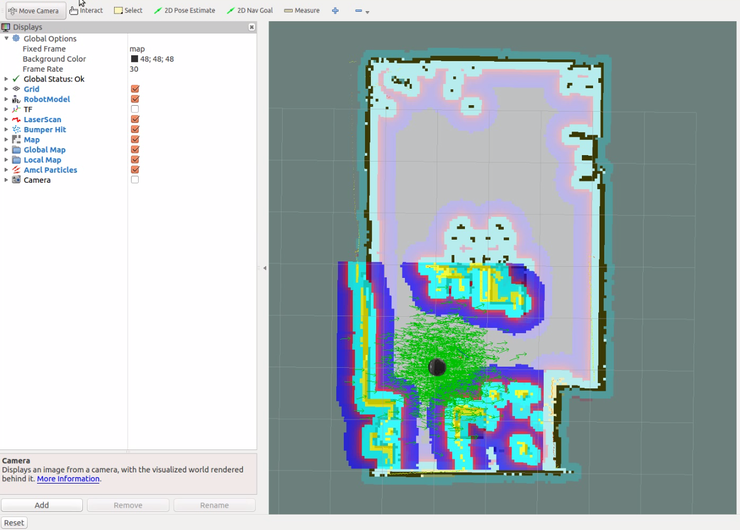
\includegraphics[width=0.9\columnwidth]{pictures/chapter11/kobuki_nav_rviz.png}
\caption{ROS 시각화 툴인 RViz의 디스플레이}
\end{figure}

이상으로 내비게이션 패키지를 사용하기 위한 필요한 모든 내용을 설명하였다. 다음 강좌에서는 costmap, Adaptive Monte Carlo Localization (AMCL), Dynamic Window Approach (DWA) 에 대한 이론 설명을 하도록 하겠다.

\newpage
%-------------------------------------------------------------------------------
\section{내비게이션 이론편}\index{내비게이션 이론편}
\label{sec:NavigationTheory}

%-------------------------------------------------------------------------------
\subsection{내비게이션 이동 가능 영역 계산을 위한 Costmap}

엔코더, 관성 센서(IMU 센서)로 부터 얻은 오도메트리와 이 정보를 기반으로 로봇의 위치 추정하여 로봇의 위치를 얻어낸다. 그리고 로봇에 장착된 거리 센서로 로봇과 장애물과의 거리를 계산한다. 내비게이션은 이 때 얻은 1)로봇 위치, 2)센서 위치, 3)장애물 위치 정보, 그리고 SLAM의 결과물로 얻은 점유 격자 지도를 4)고정 지도(static map) 로 불러와서 점유 영역(occupied area), 자유 영역(free area), 미지 영역(unknown area)에 대한 정보를 사용하게 된다. 점유 격자 지도(OGM, Occupancy Grid Map) 에 대한 자세한 설명은 섹션~\ref{sec:SlamApp}~\nameref{sec:SlamApp}(pp.\pageref{sec:SlamApp})을 다시 한번 참고하기 바란다.

내비게이션에서는 위에서 설명한 4가지 요소를 기반으로 장애물 영역, 장애물과 충돌이 예상되는 영역, 로봇이 이동 가능한 영역을 계산하게 되는데 이것을 costmap 이라고 부른다. costmap 은 다시 내비게이션의 종류에 따라 2개로 분리된다. 하나는 global\_costmap라고 하여서 전역 이동 경로 계획에서 고정 지도의 전체 영역을 대상으로 이동 계획을 수립하는데 이 때에의 출력물을 말하고, 다른 하나는 local\_costmap 이라고 한다. 이는 국부 이동 경로 계획에서 로봇을 중심으로 일부 한정된 영역에 대해 이동 계획할 때나 장애물 회피에 사용되는 지도를 말한다. 하지만, 두 costmap 은 사용 목적이 다를 뿐 지도 표현 방식에서는 동일한 지도이다. 아래에서 costmap 에 대해서 더 자세히 알아보자.

costmap 은 0 에서 255까지의 값으로 표현된다. 그 값의 의미는 아래의 도표를 참조하기 바라며 간략이 요약하면 아래와 같이 그 값에 따라 로봇이 이동 가능한 영역인지 장애물에 충돌하는 영역인지를 알 수 있게 된다. 이 각 영역 계산은 섹션~\ref{sec:NavigationApp}~\nameref{sec:NavigationApp}(pp.\pageref{sec:NavigationApp})에서 설명한 costmap 설정 파라미터에 따라 달라지게 된다.

\vspace{\baselineskip}
\begin{itemize}[leftmargin=*]
\item 000 ~ 000 : 로봇이 자유롭게 이동 가능한 자유 영역 (free area)
\item 001 ~ 127 : 충돌하지 않는 영역
\item 128 ~ 252 : 충돌 가능성이 있는 영역
\item 253 ~ 254 : 충돌 영역
\item 255 ~ 255 : 로봇이 이동 불가능한 점유 영역 (occupied area)
\end{itemize}

\begin{figure}[h]
\centering
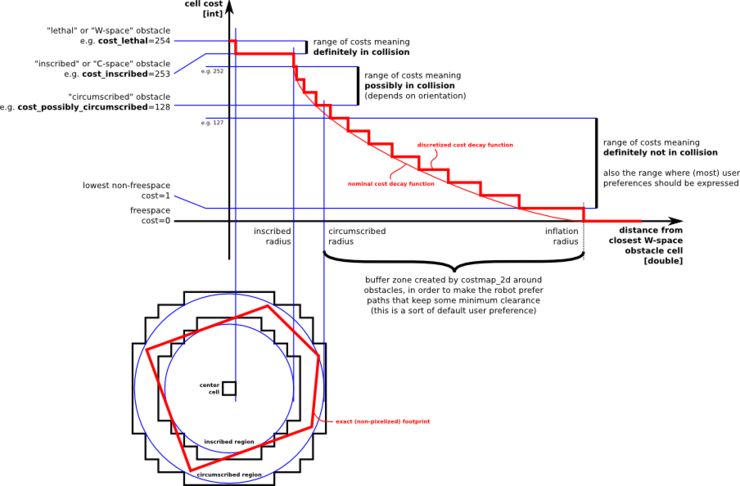
\includegraphics[width=\columnwidth]{pictures/chapter11/costmap_calculation.png}
\caption{장애물과의 거리와 costmap의 값의 관계도 (출처: \url{http://wiki.ros.org/costmap_2d?action=AttachFile&do=get&target=costmapspec.png}, CC BY 3.0)}
\end{figure}


예를 들어 costmap 을 실제로 표현하면 아래와 같이 된다. 왼쪽(그레이스케일)과 오른쪽(컬러) 은 같은 시간, 같은 위치의 상태이지만 표현 방식을 두가지로 할 수 있다는 것을 보이고 있다. 왼쪽부터 설명하자면 가운데에 거북이가 있고 그 주위로 녹색 테두리가 로봇의 모델에 해당된다. 이 녹색 라인이 실제 벽에 부딛치면 로봇은 충돌하게 된다. 빨간색은 레이저 센서에서 얻은 거리 값으로 장애물을 표시한 것이며, 검은색으로 갈수록 충돌 가능성이 높은 위치가 된다는 것을 그레이 스케일로 나태내고 있다. 오른쪽 그림도 마찬가지 인데 노란색 셀이 실제 장애물, 하늘색 영역은 로봇 중심 위치가 이 영역으로 오게되면 충돌하게 된는 지점이고 굵은 빨간색 픽셀로 경계선을 긋고 있다. 파랑색은 안전한 지역을 말한다.

\begin{figure}[h]
\centering
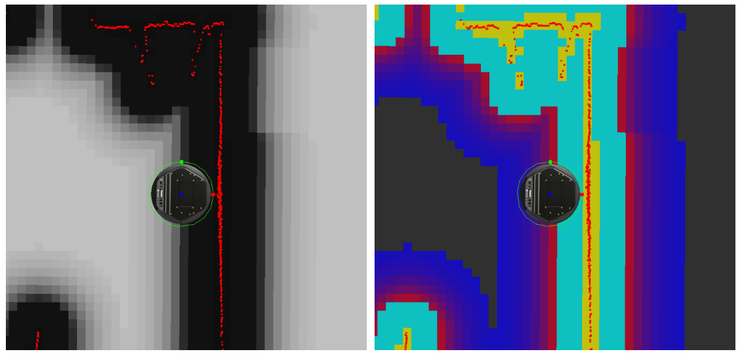
\includegraphics[width=0.8\columnwidth]{pictures/chapter11/costmap_gray.png}
\caption{costmap 표현 방식 (그레이스케일, 컬러)}
\end{figure}

%-------------------------------------------------------------------------------
\subsection{로봇 위치 추정을 위한 AMCL (Adaptive Monte Carlo Localization)}

섹션~\ref{sec:SlamTheory}~\nameref{sec:SlamTheory}(pp.\pageref{sec:SlamTheory})의 파티클 필터(particle filter) 설명에서 언급하였듯이 몬테카를로(MCL, Monte Carlo Localization) 위치추정 알고리즘은 위치 추정 분야에서 널리 사용되는 알고리즘이다. AMCL(Adaptive Monte Carlo Localization) 은 몬테카를로 위치추정 알고리즘에서 적은 수의 샘플 수를 사용하여 수행 시간을 줄여서 실시간성을 높인 몬테카를로 위치 추정의 기능 개선판이라고 볼 수 있다. 그래서, 우리는 기본이 되는 몬테카를로 위치추정(MCL)에 대해서 알아보기로 하겠다. 몬테카를로 위치 추정에 대해서는 로봇 공학에서 확률 관련 분야의 교과서로 불리우는 Sebastian Thrun 교수의 저서인 \textbf{Probabilistic Robotics}\cite{thrun2005probabilistic} 을 참조하였다. MCL 또한 Sebastian Thrun 교수와 Dieter Fox 교수의 연구결과\cite{fox1999monte}\cite{dellaert1999monte}에서 나왔으니 꼭 보기를 권장한다.

몬테카를로 위치 추정(이하 MCL)의 궁긍적인 목적은 \textbf{주어진 환경 속에서 로봇이 어디에 위치하느냐} 이다. 즉, 지도상의 $x, y, \theta$ 의 좌표를 얻어야 한다. 이를 위해서 MCL 에서는 로봇이 위치하고 있을 가능성을 확률로 계산하여 나타낸다. 우선, 시간 $t$ 에서의 로봇의 위치($x, y, \theta$)를  $x_t$ 라고 하고, 시간 $t$ 까지의 거리 센서로 부터 얻은 거리 정보를 $z_{0...t} = \{z_0, z_1, ..., z_t\}$, 시간 $t$까지의 엔코더로부터 얻은 로봇의 이동 정보를 $u_{0...t} = \{u_0, u_1, ..., u_t\}$ 라고 하였을 때, 아래와 같이 belief (베이지안 갱신 공식을 이용한 사후 확률) 를 계산한다.

\begin{equation}
  bel(x_t) = P(x_t|z_{0\cdots t},u_{0\cdots t})
\end{equation}

로봇은 하드웨어적인 오차가 생길 수 있으므로 센서모델과 이동모델을 수립하고, 베이즈 필터(bayes filter) 의  예측(prediction)과 보정(update)를 아래와 같이 거친다. 

우선 예측 단계에서는 로봇의 이동 모델 $p( x_t | x_{(t-1)}, u_{(t-1)} )$과 이전 위치에서의 확률 $bel(x_{(t-1)})$, 엔코더로부터 받은이동 정보 u 를 이용하여 다음 시간에서의 로봇의 위치 $bel'(x_t)$ 를 계산한다.

\begin{equation}
  bel'(x_t) = \int p(x_t | x_{t-1},u_{t-1})bel(x_{t-1})dx_{t-1}
\end{equation}

다음은 보정 단계인데, 이번에는 센서 모델 $p( z_t | x_t )$, 이전 위치에서의 확률 $bel(x_{(t-1)})$, 정규화 상수 $(\eta_t)$ 에타 를 이용하여 센서 정보를 기반으로 정확도를 올린 현재 위치의 확률  $bel(x_t)$을 구할 수 있다.

\begin{equation}
  bel(x_t) = \eta_t p(z_t|x_t)bel'(x_t)
\end{equation}

다음은 계산된 현재 위치의 확률 $bel(x_t)$ 를 이용하여 파티클 필터로 N 개의 파티클을 생성하여 위치 추정하는 순서인데이는 섹션~\ref{sec:SlamTheory}~\nameref{sec:SlamTheory}(pp.\pageref{sec:SlamTheory})의 파티클 필터(particle filter) 설명을 참고하기 바란다. MCL 에서는 파티클이라는 용어대신 샘플이라 하는데 전체적으로 SIR (Sampling Importance weighting Re-sampling) 과정을 거치게된다. 우선, 첫번째는 샘플링(sampling) 과정이다. 여기에서는 이전 위치에서의 확률 $bel(x_{t-1})$ 에서 로봇의 이동 모델 $p( x_t | x_{(t-1)}, u_{(t-1)}$ 을 이용하여 새로운 샘플 집합인 ${X’}_t$  를 추출하고, 이 샘플 집합 $X{’}_t$ 중 샘플 $i$ 인 ${x’}_t^{(i)}$ 와 거리 센서로 부터 얻은 거리 정보 $z_t$, 정규화상수 에타로 가중치 $\omega_t^{(i)}$ 를 구한다. 

\begin{equation}
  \omega_t^{(i)} = \eta p(z_t|x_t^{\prime(i)})
\end{equation}

마지막으로 리샘플링 과정에서는 샘플 ${x’}_t^{(i)}$와 가중치 $w_t^{(i)}$ 를 이용하여 $N$ 개의 새로운 $X_t$ 샘플링 (파티클) 집합을 만들어 내는 것이다. 

\begin{equation}
  X_t = \{x_t^{(j)} | j=1 \cdots N\} \sim \{x_t^{\prime(i)},\omega_t^{(i)}\}
\end{equation}

이렇게 SIR 과정을 되풀이 하면서 파티클을 이동시켜 가고, 로봇 위치 추정치는 그 정확도를 높여 가게 된다. 예를들어 아래의 그림과 같이 $t_1, t_2, t_3, t_4$ 로 갈 수록 점점 수렴하는 과정을 볼 수 있을 것이다. 마지막으로 이 모든 과정을 Sebastian Thrun 교수의 저서 "Probabilistic Robotics"  에서는 자세히 설명하고 있다. 시간이 된다면 꼭 찾아보기를 추천한다. 

\begin{figure}[h]
\centering
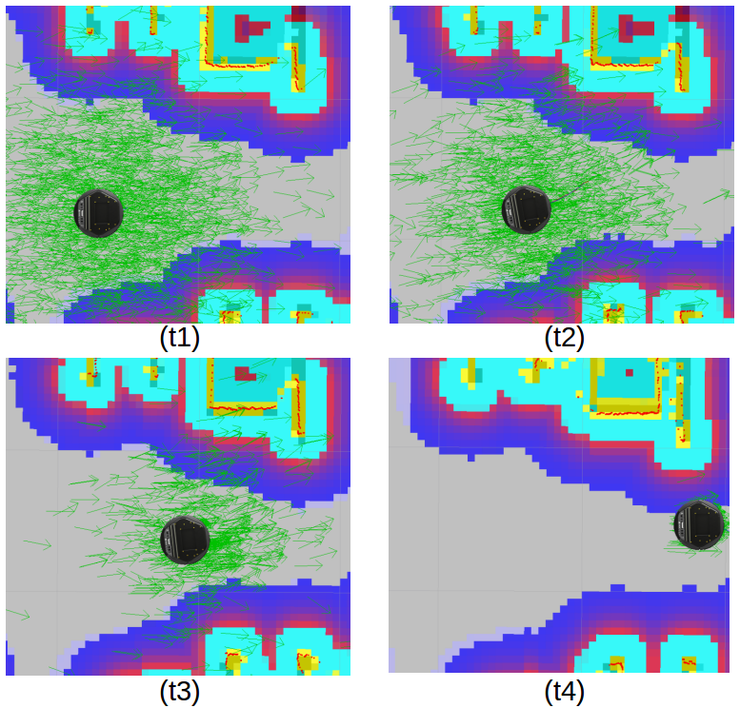
\includegraphics[width=0.9\columnwidth]{pictures/chapter11/amcl.png}
\caption{로봇 위치 추정을 위한 AMCL 과정}
\end{figure}

이상으로 내비게이션 이론편을 마치기로 한다. 이동 경로 계획 및 장애물 회피할 때 많이 사용되는 Dynamic Window Approach (DWA) 에 대한 설명을 기한내에 못했는데 다음 기회에 이는 추가로 설명하도록 하겠다.

%-------------------------------------------------------------------------------


